\section{解析}
実験で得られたデータからははっきりと波うつパターンが見て取れる。この章ではその波模様をいくつかの要素に分解し、それぞれについて理論的に説明できるかどうかを考えてゆく。私たちは望んだ干渉の結果を見ることができたのか。

\subsection{波の分解}

\ref{Resonance_sec}章で述べたように、干渉パターンは最も一般的には、共鳴からのずれを表すパラメータ$\epsilon$と中性子の速度$v$に依存した係数$N_1,N_2,N_3$を用いて
\begin{equation}
I=N_1-N_2\cos\left(\frac{2}{v}(\omega d'-\epsilon L')\right) -N_3\sin\left(\frac{2}{v}(\omega d'-\epsilon L')\right) \label{Discussion_theory_ippan}
\end{equation}
と表せる。ここで$\omega$は位相シフタコイルの磁場$B_p$を用いて$\omega=|\mu_n|B_p$と表される量であり、$d',L'$はそれぞれ位相シフタコイルの幅、2つのスピンフリッパー間距離である。さらに$N_4=\sqrt{N_2^2+N_3^2}$として
\begin{equation}
\cos \phi=\frac{N_2}{N_4}, \quad \sin \phi=\frac{N_3}{N_4}
\end{equation}
で$\phi$を定義すれば、干渉パターンは
\begin{equation}
I=N_1-N_4\cos\left(\frac{2}{v}(\omega d'-\epsilon L')-\phi\right)\label{Discussion_theory_ippan2}
\end{equation}
と書き直される。このように書くと実験データをフィッティングして得られる4つのパラメータと理論式を対応づけることができる。すなわち、実験で得られた波模様を位相シフタコイルに流した電流$I_p$に対して
\begin{equation}
I=D-A\cos(B\cdot I_p+C)
\end{equation}
という関数でフィッティングしたときの4つのパラメータ$A,B,C,D$は理論と
\begin{comment}
\renewcommand{\arraystretch}{1.5}
\begin{equation}
\begin{array}{l}
A \leftrightarrow N_4\\
B \leftrightarrow \dfrac{2\omega d'}{v(-I_p)}\\
C \leftrightarrow \dfrac{2\epsilon L'}{v} +\phi \\
D \leftrightarrow N_1
\end{array}
\end{equation}
\renewcommand{\arraystretch}{1}
\end{comment}
\begin{align}
A \leftrightarrow N_4&&B \leftrightarrow \dfrac{2\omega d'}{v(-I_p)}&&C \leftrightarrow \dfrac{2\epsilon L'}{v} +\phi&&D \leftrightarrow N_1
\end{align}
と対応づくことがわかる。なお、$I_p$は鉛直下向きに磁場が発生する向きを正としたため、$B,C$については理論式(\ref{Discussion_theory_ippan})のコサインの中身にマイナスをかけて対応づけておく。

なお、実験で得られたデータはある波長領域について積分したものであるため、ひとつの波長に対して定められた理論式(\ref{Discussion_theory_ippan})とは厳密には対応づかない。しかし十分狭い波長領域で見れば、近似的に領域の中心の波長に対する理論式とその波長領域での実験値を対応づけることができる。このことの詳しい議論は後で行う。

ここで行ったことの要は、単に実験と理論を対応づけたということではなく、波模様というあいまいな概念を輪郭の明確な4つの要素に分解したことにある。これによって私たちは奇妙にゆれる波に惑わされることなく、個々の要素について着実に考えてゆくことができる。

\subsection{$B$}
\paragraph{パラメータ$B$の意味}
$B$には干渉という現象のエッセンスが凝縮されている。上では干渉パターンの最も一般的な形を見たが、逆に最も特殊な場合を見てみよう。それは共鳴条件()が満たされている中で、$\pi/2$フリップ条件()を満たす速度の中性子を対象とした場合である。そのときは$N_1=1/2,N_2=1/2,N_3=0,\epsilon=0$であるから、干渉パターンは
\begin{equation}
I=\frac{1}{2}\left(1-\cos\frac{2\omega d'}{v}\right) \label{Discussion_theory_simple}
\end{equation}
となる。このように、非常にシンプルな場合を考えてもスピン上下の位相差を表す$B$の部分の形は変わらない。そのような意味で$B$は干渉の本質を担っている。

\paragraph{理論からのアプローチ}
理論的には$B$は$2\omega d'/v(-I_p)$と書かれるが、$\omega \propto -I_p$であって、具体的に書けば
\begin{align}
\omega d'=\frac{|\mu_n|B_p d'}{\hbar}=\frac{(-I_p)|\mu_n| b_p d'}{\hbar}
\end{align}
となる。ここで$b_p$は位相シフタコイルに1Aの電流を流したときに発生する磁束密度。なおこの章では実験値と理論値を比較する必要からSI単位系を用い、$\hbar$も明記する。さらに位相シフタコイルによる磁場は空間的に一様ではないため、実際は粒子の軌道に沿った積分で表す必要がある:
\begin{equation}
b_p d' \rightarrow \int b_p(x) dx
\end{equation}

次の図\ref{Discussion_fig_PhaseShifterSimulation}は位相シフタコイルに1Aの電流を流したときの磁場分布シミュレーション結果である。%またシフタコイルの中心($y=z=0$)を通ったときの$x$軸に沿っての磁場分布を図\ref{Discussion_fig_PSS_danmen}に表す。
このシミュレーションを用いて$\int b_p(x) dx$を計算すると、シフタコイルの中心($y=z=0$)を通ったときの積分値は
\begin{equation}
\int b_p(x) dx =2.75 \times 10^{-5} \mathrm{T\cdot m/A}
\end{equation}
となった。なお積分範囲は実際の配置と図\ref{Discussion_fig_PSS_danmen}より、$-20$cmから$20$cmとした。また粒子の経路が$y$方向や$z$方向にずれたときの積分値は図\ref{Discussion_fig_PSS_zure}のようになった。ビームの幅は20mm程度であるから、中性子の経路による積分値のずれは1\%程度に抑えられると考えられる。そこで今後の解析には中心での値を用いることにする。
\begin{figure}[h]
\centering
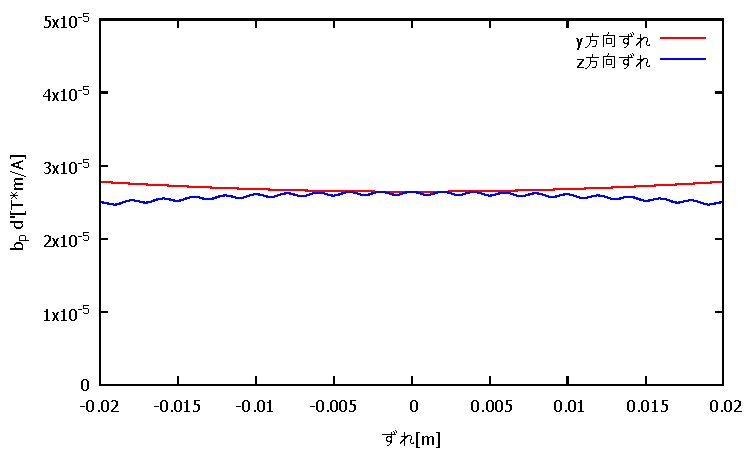
\includegraphics[width=9cm]{discussion/B/bd.pdf}
\caption{$y,z$方向のずれによる影響} \label{Discussion_fig_PSS_zure}
\vspace{-5mm}
\end{figure}

ゆえに$B$の理論値は
\begin{equation}
\frac{2\omega d'}{v(-I_p)}=2\frac{|\mu_n|\int b_p dx}{\hbar v}=2\frac{|\mu_n|\int b_p dx}{\hbar}\frac{m}{h}\lambda=1.27 \cdot \lambda \ [1/A] \label{Discussion_theory_B}
\end{equation}
となる。ただし$\lambda$[\AA]は中性子の波長。 

\begin{figure}[H]
%\begin{minipage}{0.5\hsize}
\begin{center}
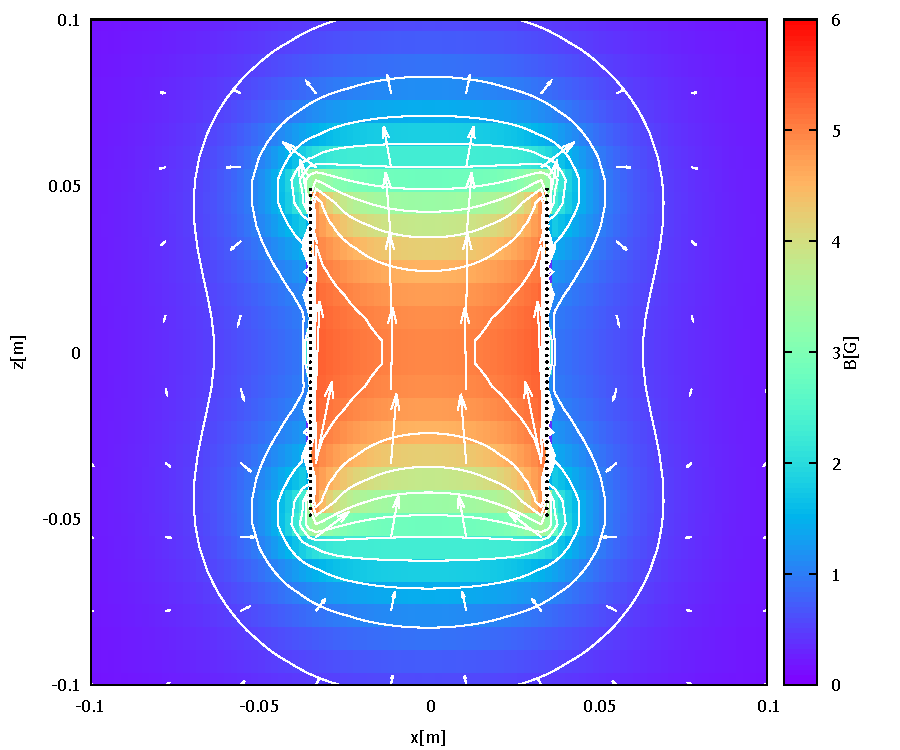
\includegraphics[width=9cm]{discussion/B/coil11_image1.pdf}
\vspace{-1mm}
\subcaption{横から}
\vspace{-3mm}
%\end{minipage}
%\begin{minipage}{0.5\hsize}
%\centering
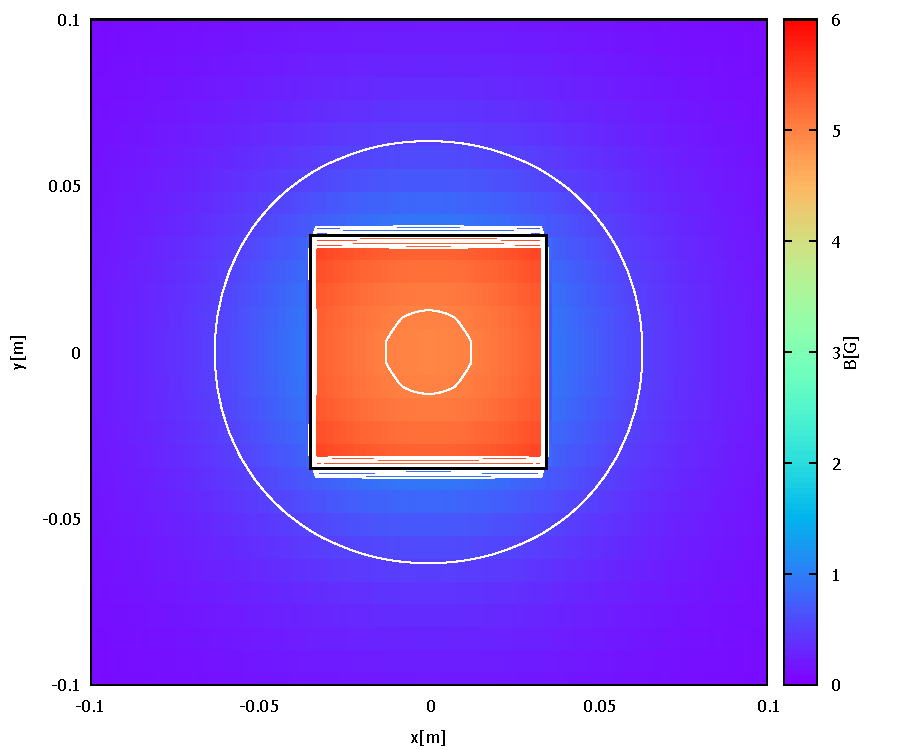
\includegraphics[width=9cm]{discussion/B/coil11_image2.pdf}
\vspace{-1mm}
\subcaption{上から}
\vspace{-3mm}
%\end{minipage}\\
%\begin{center}
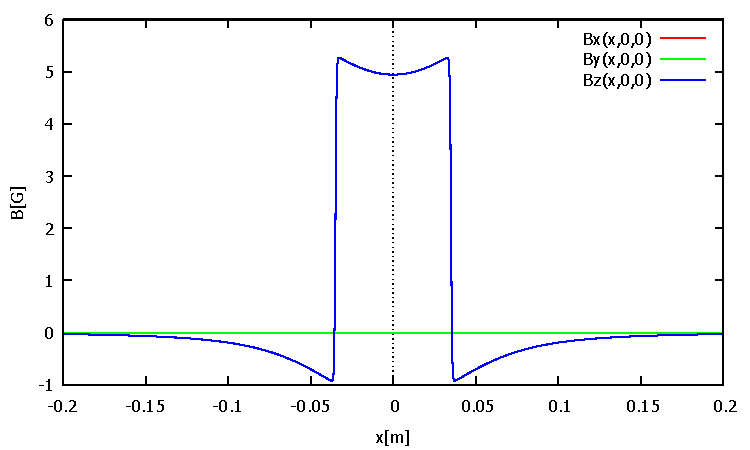
\includegraphics[width=9cm]{discussion/B/coil11_danmen1.pdf}
\vspace{-1mm}
\subcaption{中心($y=z=0$)を通ったとき}
\vspace{-3mm}
\end{center}
%\end{center}
\caption{位相シフタコイル磁場分布シミュレーション} \label{Discussion_fig_PhaseShifterSimulation}
%\vspace{-1cm}
\end{figure}

\paragraph{実験結果・解析}
以下の表\ref{Discussion_tbl_B}に波長領域$\lambda \pm 0.07 \AA$における実験データから得られた$B$の値と式(\ref{Discussion_theory_B})から得られる理論値を示す。なお理論値には中性子の経路による誤差1\% が含まれるとした。また表\ref{Discussion_tbl_B}の結果を図\ref{Discussion_fig_B}に表す。図、表からわかるように全ての波長領域でパラメータ$B$の実験値と理論値はよく一致しており、多くの波長において誤差の範囲で一致している。

\begin{figure}[h]
\begin{minipage}{0.35\hsize}
\centering
\makeatletter
\def\@captype{table}
\makeatother
\caption{各波長領域におけるパラメータ$B$の実験値と理論値} \label{Discussion_tbl_B}
\begin{tabular}{lll}
$\lambda$[\AA] &  $B(実験)$ &   理論値 \\ \hline
3.06  & 4.18  $\pm$ 0.05  & 3.90  $\pm$ 0.04  \\
3.21  & 4.14  $\pm$ 0.05  & 4.08  $\pm$ 0.04  \\
3.35  & 4.32  $\pm$ 0.05  & 4.27  $\pm$ 0.04  \\
3.42  & 4.42  $\pm$ 0.04  & 4.36  $\pm$ 0.04  \\
3.50  & 4.52  $\pm$ 0.05  & 4.45  $\pm$ 0.04  \\
3.56  & 4.63  $\pm$ 0.07  & 4.54  $\pm$ 0.05  \\
3.66  & 4.74  $\pm$ 0.07  & 4.66  $\pm$ 0.05  \\
3.75  & 4.77  $\pm$ 0.09  & 4.78  $\pm$ 0.05  \\
3.86  & 5.09  $\pm$ 0.09  & 4.91  $\pm$ 0.05  \\
4.00  & 5.15  $\pm$ 0.08  & 5.10  $\pm$ 0.05  \\
4.15  & 5.16  $\pm$ 0.18  & 5.28  $\pm$ 0.05  \\
4.29  & 3.36  $\pm$ 0.17  & 5.47  $\pm$ 0.05  \\ \hline
\end{tabular}
\end{minipage}
\begin{minipage}{0.65\hsize}
\centering
\vspace{2.5cm}
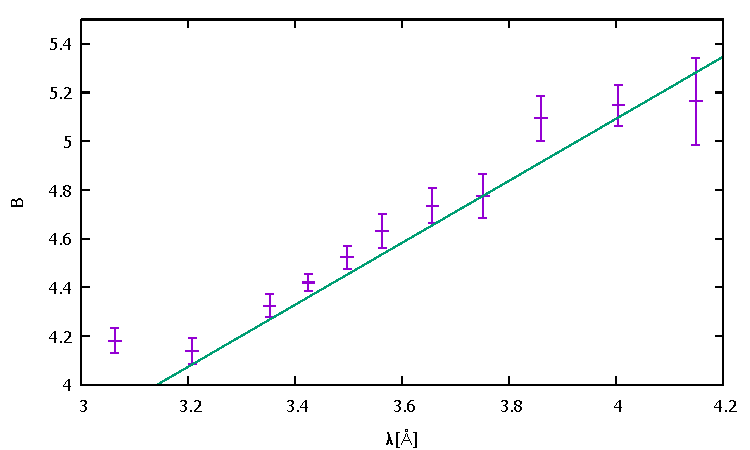
\includegraphics[width=10cm]{discussion/B/B_F.pdf}
\caption{各波長領域に対する$B$} \label{Discussion_fig_B}
\end{minipage}
\end{figure}

\paragraph{結論}
パラメータ$B$こそスピン干渉の本質であり、それが干渉のみられた全ての波長領域で理論値とよく一致したということは、私たちが望みのものを手に入れたということを示唆している。目的は果たされた。

\subsection{$C$}
\paragraph{パラメータ$C$の意味}
干渉においてパラメータ$B$の次に重要な意味をもつパラメータは$C$であろう。最もシンプルな場合(\ref{Discussion_theory_simple})を考えると、理論的にはパラメータ$C$に対応する位相のシフトは入ってこなかった:
\begin{equation}
I=\frac{1}{2}\left(1-\cos\frac{2\omega d'}{v}\right)
\end{equation}
$C$の対応物$2\epsilon L'/v +\phi$は、どちらの項も$\epsilon=0$のときゼロとなるためである。すなわちパラメータ$C$は共鳴からのずれに依存する。パラメータ$C$を分析することで、共鳴からのずれを知ることができる。

\paragraph{理論からのアプローチ}
理論的には$C$は$2\epsilon L'/v +\phi$に対応し、$\cos\phi=N_2/N_4,\sin\phi=N_3/N_4$であった。\ref{Resonance_sec}章より
\begin{align}
&N_2 = 2\left(\frac{\omega_r}{\omega_A}\right)^2\sin^2\frac{\omega_A}{v}d \left(\cos^2 \frac{\omega_A}{v}d -\left(\frac{\epsilon}{\omega_A}\right)^2 \sin^2 \frac{\omega_A}{v}d\right) \\
&N_3 = 4\frac{\epsilon}{\omega_A} \left(\frac{\omega_r}{\omega_A}\right)^2\sin^3\frac{\omega_A}{v}d \cos \frac{\omega_A}{v}d
\end{align}
であるから$N_4$は
\begin{equation}
N_4=\sqrt{N_2^2+N_3^2}=2\left(\frac{\omega_r}{\omega_A}\right)^2\sin^2\frac{\omega_A}{v}d \left(\cos^2\frac{\omega_A}{v}d+\left(\frac{\epsilon}{\omega_A}\right)^2\sin^2\frac{\omega_A}{v}d\right)
\end{equation}
と書ける。ここで$\omega_A=\sqrt{\epsilon^2+\omega_r^2}$であり、$d$はフリッパーの幅である。よって
\begin{align}
\cos\phi&=\frac{\cos^2 \frac{\omega_A}{v}d -\left(\frac{\epsilon}{\omega_A}\right)^2 \sin^2 \frac{\omega_A}{v}d}{\cos^2\frac{\omega_A}{v}d+\left(\frac{\epsilon}{\omega_A}\right)^2\sin^2\frac{\omega_A}{v}d} \\
\sin\phi&=\frac{2\frac{\epsilon}{\omega_A}\sin\frac{\omega_A}{v}d \cos \frac{\omega_A}{v}d}{\cos^2\frac{\omega_A}{v}d+\left(\frac{\epsilon}{\omega_A}\right)^2\sin^2\frac{\omega_A}{v}d}
\end{align}
であり、確かに$\epsilon=0$のとき$\phi=0$となる。次の図\ref{Discussion_fig_phi}に$\epsilon/\omega_z=0,0.1,0.3,0.5,1.0$のときの中性子の波長$\lambda$に対する$\phi$の理論値を表す。ただし$\omega_r/\omega_z=0.25,B_z=12.8\,\mathrm{G}$とした。
\begin{figure}[h]
\centering
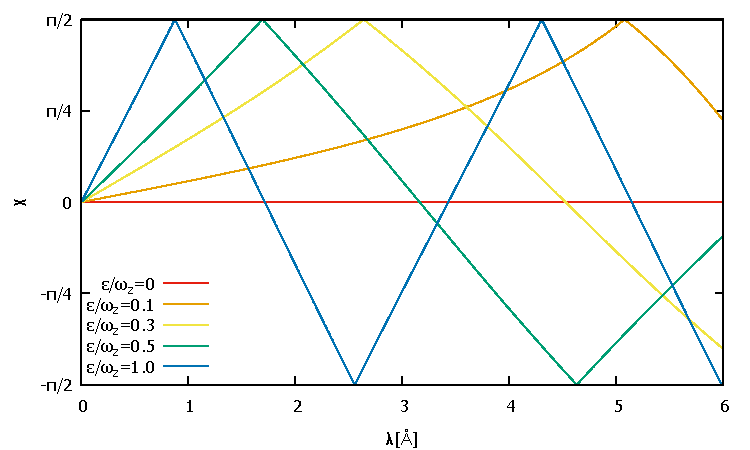
\includegraphics[width=10cm]{discussion/C/chi.pdf}
\caption{中性子の波長$\lambda$に対する$\phi$} \label{Discussion_fig_phi}
\end{figure}

これを実験値と比べるためにはもう一工夫必要となる。理論では上流と下流のスピンフリッパーで$\omega_r$の値は等しいとしていた。しかし、実際に測定データから得られた$\omega_r$は上流と下流で異なっていた(\ref{Resonance_sec}章参照)。%上流、下流フリッパーの$\omega_r$をそれぞれ$\omega_{r1},\omega_{r2}$とすると$\omega_r/2\pi=8.7\pm0.1\,\mathrm{kHz},
そこで上流、下流フリッパーの$\omega_r$をそれぞれ$\omega_{r1},\omega_{r2}$として、2つのフリッパーで$\omega_r$が異なる場合も含めた干渉パターンの式を求めると、式の形は$\omega_r$が等しい場合(\ref{Discussion_theory_ippan})と同じで、係数が
\begin{align}
&N_1 = \left(\cos^2 \frac{\omega_{A1}}{v}d +\left(\frac{\epsilon}{\omega_{A1}}\right)^2\sin^2 \frac{\omega_{A1}}{v}d\right)\left(\cos^2 \frac{\omega_{A2}}{v}d+\left(\frac{\epsilon}{\omega_{A2}}\right)^2 \sin^2 \frac{\omega_{A2}}{v}d\right)\\ \notag
&\hspace{7cm}+\left(\frac{\omega_{r1}}{\omega_{A1}}\right)^2\left(\frac{\omega_{r2}}{\omega_{A2}}\right)^2 \sin^2 \frac{\omega_{A1}}{v}d \sin^2 \frac{\omega_{A2}}{v}d\\
&N_2 = 2\frac{\omega_{r1}}{\omega_{A1}}\frac{\omega_{r2}}{\omega_{A2}}\sin\frac{\omega_{A1}}{v}d\sin\frac{\omega_{A2}}{v}d \left(\cos \frac{\omega_{A1}}{v}d\cos \frac{\omega_{A2}}{v}d -\frac{\epsilon}{\omega_{A1}}\frac{\epsilon}{\omega_{A2}} \sin \frac{\omega_{A1}}{v}d\sin \frac{\omega_{A2}}{v}d\right) \\
&N_3 = 2\frac{\omega_{r1}}{\omega_{A1}}\frac{\omega_{r2}}{\omega_{A2}}\sin\frac{\omega_{A1}}{v}d\sin\frac{\omega_{A2}}{v}d \left(\frac{\epsilon}{\omega_{A1}}\sin \frac{\omega_{A1}}{v}d\cos \frac{\omega_{A2}}{v}d +\frac{\epsilon}{\omega_{A2}} \sin \frac{\omega_{A1}}{v}d\cos \frac{\omega_{A2}}{v}d\right)
\end{align}\label{Discussion_theory_ippanippan}
となる。ここで$\omega_{Ai}=\sqrt{\epsilon^2+\omega_{ri}^2} \ (i=1,2)$である。これでパラメータ$C$について実験値と理論値を比較する準備が整った。

\paragraph{実験結果}
以下の表\ref{Discussion_tbl_C}に波長領域$\lambda \pm 0.07 \AA$における実験データから得られた$C$の値を示し、中心波長$\lambda$と$C$の関係を図\ref{Discussion_fig_C}に表す。
\begin{figure}[h]
\begin{minipage}{0.35\hsize}
\centering
\makeatletter
\def\@captype{table}
\makeatother
\caption{各波長領域におけるパラメータ$C$の実験値} \label{Discussion_tbl_C}
\begin{tabular}{ll}
$\lambda$[\AA] &  $C(実験)$\\ \hline
3.06 	&	1.12 	$\pm$	0.09 \\
3.21 	&	1.61 	$\pm$	0.09 \\
3.35 	&	1.90 	$\pm$	0.07 \\
3.42 	&	2.04 	$\pm$	0.06 \\
3.50 	&	2.14 	$\pm$	0.08 \\
3.56 	&	2.27 	$\pm$	0.12 \\
3.66 	&	2.50 	$\pm$	0.12 \\
3.75 	&	2.52 	$\pm$	0.14 \\
3.86 	&	2.87 	$\pm$	0.16 \\
4.00 	&	3.12 	$\pm$	0.15 \\
4.15 	&	3.72 	$\pm$	0.31 \\
4.29 	&	3.76 	$\pm$	0.28 \\ \hline
\end{tabular}
\end{minipage}
\begin{minipage}{0.65\hsize}
\centering
\vspace{2.5cm}
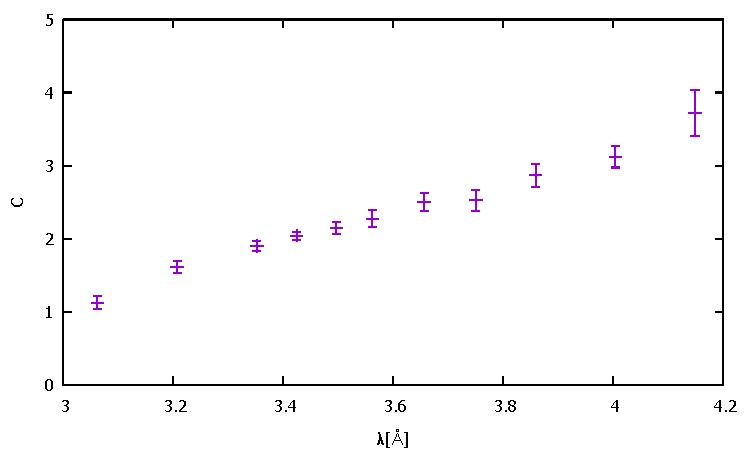
\includegraphics[width=10cm]{discussion/C/C_F.pdf}
\caption{中心波長$\lambda$と$C$の関係} \label{Discussion_fig_C}
\end{minipage}
\end{figure}

\paragraph{解析}
$\epsilon/\omega_z$をフィッティングパラメータとして実験値をフィッティングすることを考える。このときフィッティング関数は$2\epsilon L'/v +\phi$であるが、正確には$2n\pi$(n:整数)の不定性が存在する。そこでフィッティング関数として次の形を用い、$n=-3,-2,-1,0,1,2$の各場合についてフィッティングを行った。
\begin{equation}
2\epsilon L'/v +\phi+2n\pi
\end{equation}
なお、各種パラメータには実測と測定データから求めた次の値を用いた。
\begin{table}[h]
\centering
\caption{各種パラメータ}\label{Discussion_tbl_parameter}
\begin{tabular}{ccccc}
$\omega_{r1}/2\pi$[kHz]&$\omega_{r2}/2\pi$[kHz]&$\omega_{z}/2\pi$[kHz]&$d$[mm]&$L'$[mm]\\ \hline
4.4&4.8&18.7&30&273
\end{tabular}
\end{table}

次の表\ref{Discussion_tbl_Cfit}に各$n$におけるフィッティングの結果を示す。カイ二乗が最も小さくなった$n=-1$のときについてフィッティング結果を図\ref{Discussion_fig_Cfit}に表す。

\paragraph{結論}
パラメータ$C$は共鳴からのずれと関係づく。$\epsilon/\omega_z=0.131\pm0.001$とすると、干渉のみられた全ての波長領域でパラメータ$C$の実験値は理論値とよく一致した。すなわち今回の実験における共鳴からのずれは$\epsilon/\omega_z=0.131\pm0.001$程度であったと推測される。

\begin{table}[H]
\centering
\caption{$n=-3,-2,-1,0,1,2$に対するフィッティング結果}\label{Discussion_tbl_Cfit}
\begin{tabular}{ccc}
$n$&$\epsilon/\omega_z$&reduced $\chi^2$\\ \hline
$-3$	&$0.364 \pm0.004$ 	&56.8 \\
$-2$	&$0.237 \pm0.002$ 	&9.43 \\
$-1$	&$0.131 \pm0.001$ 	&2.16 \\
$0$	&$0.033 \pm0.002$ 	&14.1 \\
$1$	&$-0.066 \pm0.004$ 	&76.1 \\
$2$	&$-0.165 \pm0.006$ 	&182\\ \hline
\end{tabular}
\end{table}
\begin{figure}[h]
\centering
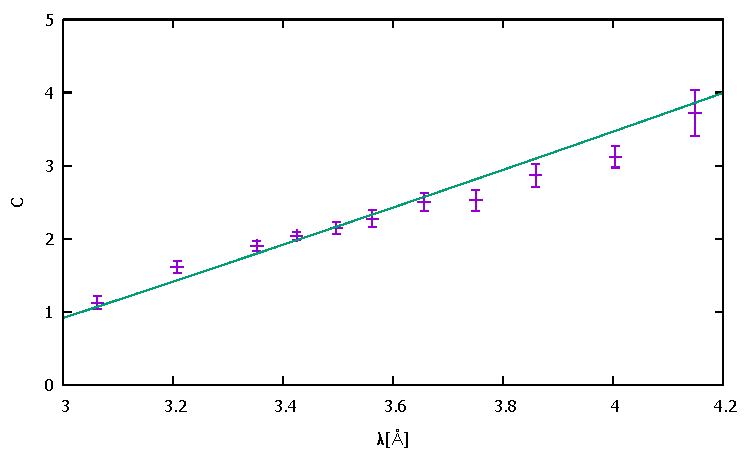
\includegraphics[width=10cm]{discussion/C/C_F_fit.pdf}
\caption{$n=-1$のときのフィッティング結果}\label{Discussion_fig_Cfit}
\end{figure}

\subsection{$D$}
\paragraph{パラメータ$D$の意味}
パラメータ$D$は干渉の波模様がどこを中心に振動しているかを表す。パラメータ$D$は波の位相ではなく波の高さに関係した量であるという点で、前述のパラメータ$B$や$C$と異なる。波の位相については粒子数の相対的な差から情報を得ることができるが、波の高さについては粒子数の絶対値が影響する。したがってパラメータ$D$からはパラメータ$B$,$C$からは知り得なかった粒子数の絶対値に関係した情報を得ることができる。

\paragraph{理論からのアプローチ}
理論的には$D$は$N_1$に対応する。2つのフリッパーで$\omega_r$が異なる場合も含めた最も一般的な$N_1$の表式は次の通りであった:
\begin{align}
&N_1 = \left(\cos^2 \frac{\omega_{A1}}{v}d +\left(\frac{\epsilon}{\omega_{A1}}\right)^2\sin^2 \frac{\omega_{A1}}{v}d\right)\left(\cos^2 \frac{\omega_{A2}}{v}d+\left(\frac{\epsilon}{\omega_{A2}}\right)^2 \sin^2 \frac{\omega_{A2}}{v}d\right)\\ \notag
&\hspace{7cm}+\left(\frac{\omega_{r1}}{\omega_{A1}}\right)^2\left(\frac{\omega_{r2}}{\omega_{A2}}\right)^2 \sin^2 \frac{\omega_{A1}}{v}d \sin^2 \frac{\omega_{A2}}{v}d
\end{align}
これを種々の$\epsilon/\omega_z$に対して波長を横軸として図示すると図\ref{Discussion_fig_N1}のようになる。各種パラメータには表\ref{Discussion_tbl_parameter}の値を用いた。
\begin{figure}[h]
\centering
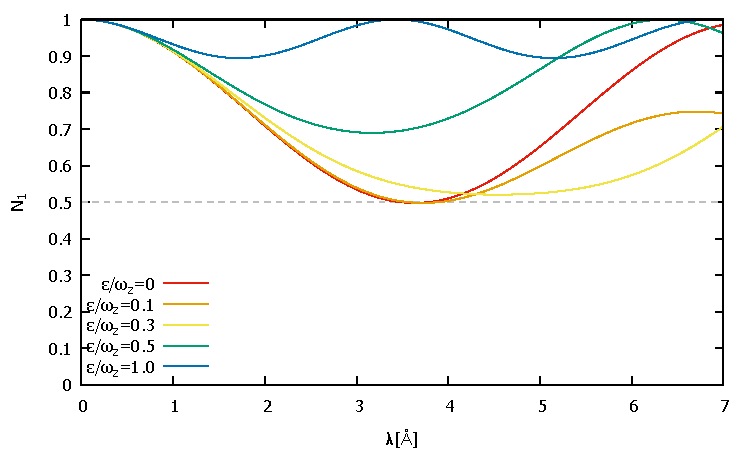
\includegraphics[width=10cm]{discussion/D/N1.pdf}
\caption{中性子の波長$\lambda$に対する$N_1$}\label{Discussion_fig_N1}
\end{figure}

\paragraph{実験結果}
以下の表\ref{Discussion_tbl_D}に波長領域$\lambda \pm 0.07 \AA$における実験データから得られた$D$の値を示し、中心波長$\lambda$と$D$の関係を図\ref{Discussion_fig_D}に表す。
\begin{figure}[H]
\begin{minipage}{0.35\hsize}
\centering
\makeatletter
\def\@captype{table}
\makeatother
\caption{各波長領域におけるパラメータ$D$の実験値} \label{Discussion_tbl_D}
\begin{tabular}{ll}
$\lambda$[\AA] &  $D(実験)$\\ \hline
3.06 	&	0.61 	$\pm$	0.05 	\\
3.21 	&	0.63 	$\pm$	0.05 	\\
3.35 	&	0.53 	$\pm$	0.04 	\\
3.42 	&	0.59 	$\pm$	0.05 	\\
3.50 	&	0.63 	$\pm$	0.05 	\\
3.56 	&	0.59 	$\pm$	0.05 	\\
3.66 	&	0.58 	$\pm$	0.05 	\\
3.75 	&	0.66 	$\pm$	0.06 	\\
3.86 	&	0.69 	$\pm$	0.07 	\\
4.00 	&	0.91 	$\pm$	0.10 	\\
4.15 	&	0.79 	$\pm$	0.09 	\\
4.29 	&	0.81 	$\pm$	0.09 	\\ \hline
\end{tabular}
\end{minipage}
\begin{minipage}{0.65\hsize}
\centering
\vspace{2.5cm}
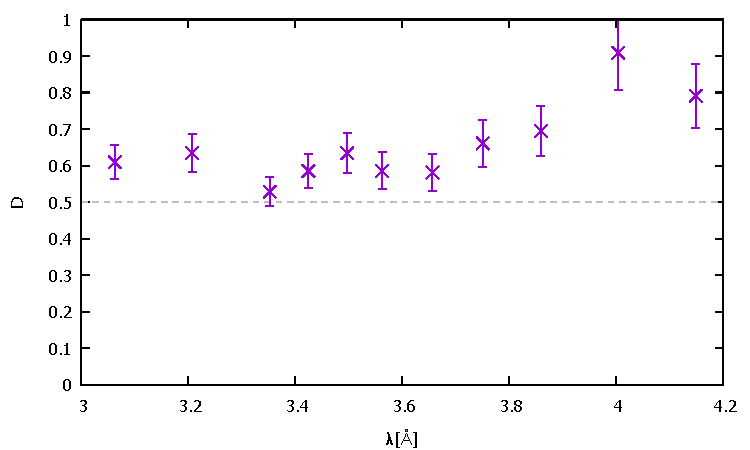
\includegraphics[width=10cm]{discussion/D/D_F.pdf}
\caption{中心波長$\lambda$と$D$の関係} \label{Discussion_fig_D}
\end{minipage}
\end{figure}

\paragraph{解析}
パラメータ$C$に対する考察の結果から$\epsilon/\omega_z=0.131$としたときの$D$の理論値を実験値と共に図\ref{Discussion_fig_D_N1}に表す。このときreduced$\chi^2=74/12=6.2$となり、理論値と実験値の一致はあまりよくない。全ての波長において実験値は理論値よりも上にずれている。これは粒子数の変動の中心が数の多い方へシフトしていることを意味しており、バックグラウンドの存在が示唆される。
\begin{figure}[h]
\centering
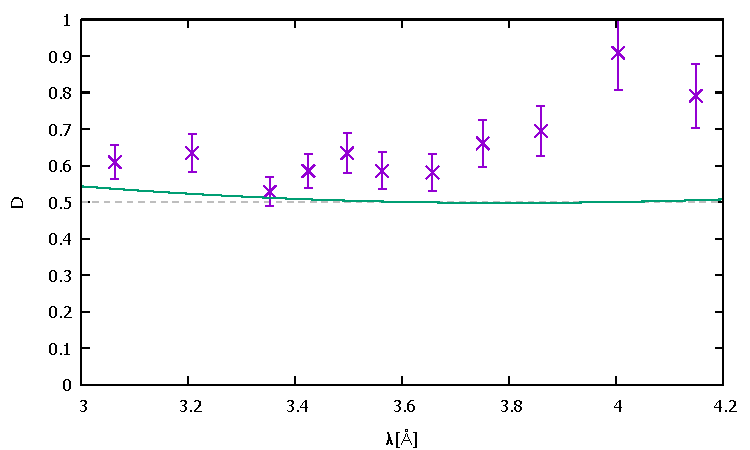
\includegraphics[width=10cm]{discussion/D/D_F_N1.pdf}
\caption{波長に対する$D$の実験値と$\epsilon/\omega_z=0.131$のときの理論値}\label{Discussion_fig_D_N1}
\end{figure}

\paragraph{結論}
パラメータ$D$は干渉波が振動する中心の高さを表し、パラメータ$B$や$C$からは知り得なかった粒子数の絶対値に関する情報を教えてくれる。$D$の実験値が理論値と比べて大きくなっていることはバックグラウンドの存在を示唆している。バックグラウンドに関する詳しい議論は後にまわす。

\subsection{$A$}
\paragraph{パラメータ$A$の意味}
パラメータ$A$は干渉の波模様の振幅を表す。パラメータ$A$は$D$と同様に波の高さに関係した量であり、絶対的な粒子数に関する情報を持つ。一方で位相のずれた波が重なるとうなりが生じて振幅は変化する。その意味でパラメータ$A$は位相に関する情報も持っているといえる。

\paragraph{理論からのアプローチ}
理論的には$A$は$N_4$に対応する。その具体的な表式は式(\ref{Discussion_theory_ippanippan})より
\begin{align}
N_4&=\sqrt{N_2^2+N_3^2} \notag \\
&=2\frac{\omega_{r1}}{\omega_{A1}}\frac{\omega_{r2}}{\omega_{A2}}\sin\frac{\omega_{A1}}{v}d\sin\frac{\omega_{A2}}{v}d\sqrt{\left(\cos^2 \frac{\omega_{A1}}{v}d +\left(\frac{\epsilon}{\omega_{A1}}\right)^2\sin^2 \frac{\omega_{A1}}{v}d\right)\left(\cos^2 \frac{\omega_{A2}}{v}d+\left(\frac{\epsilon}{\omega_{A2}}\right)^2 \sin^2 \frac{\omega_{A2}}{v}d\right)}
\end{align}
である。これを種々の$\epsilon/\omega_z$に対して波長を横軸として図示すると図\ref{Discussion_fig_N4}のようになる。各種パラメータには表\ref{Discussion_tbl_parameter}の値を用いた。図\ref{Discussion_fig_N4}は波長に対する$N_1$を描いた図\ref{Discussion_fig_N1}を0.5を境に反転したように見える。実際、$\omega_{r1}=\omega_{r2}$のときは$N_1+N_4=1$が厳密になりたつ。つまり上流下流のスピンフリッパーで$\omega_r$が等しいときは共鳴のいかんに関わらず常に干渉の波の頂上は1に達する(図\ref{Resonance_fig_interference}参照)。
\begin{figure}[H]
\centering
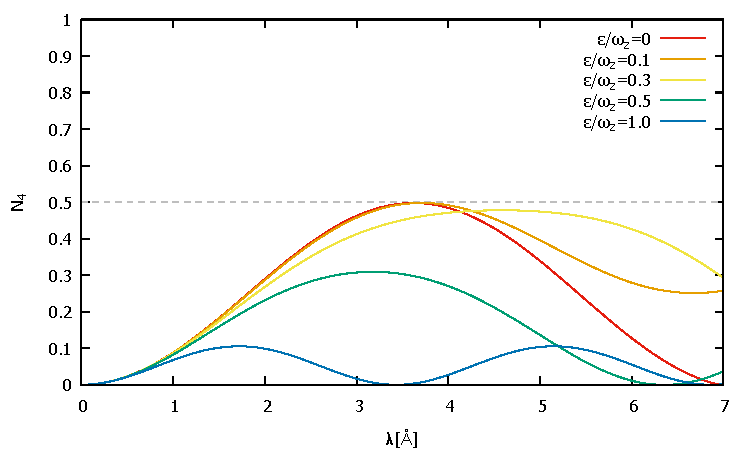
\includegraphics[width=10cm]{discussion/A/N4.pdf}
\caption{中性子の波長$\lambda$に対する$N_4$}\label{Discussion_fig_N4}
\end{figure}

\paragraph{実験結果}
以下の表\ref{Discussion_tbl_A}に波長領域$\lambda \pm 0.07 \AA$における実験データから得られた$A$の値を示し、中心波長$\lambda$と$A$の関係を図\ref{Discussion_fig_A}に表す。
\begin{figure}[H]
\begin{minipage}{0.35\hsize}
\centering
\makeatletter
\def\@captype{table}
\makeatother
\caption{各波長領域におけるパラメータ$A$の実験値} \label{Discussion_tbl_A}
\begin{tabular}{ll}
$\lambda$[\AA] &  $A(実験)$\\ \hline
3.06 	&	0.21 	$\pm$	0.02 	\\
3.21 	&	0.27 	$\pm$	0.03 	\\
3.35 	&	0.25 	$\pm$	0.02 	\\
3.42 	&	0.28 	$\pm$	0.03 	\\
3.50 	&	0.30 	$\pm$	0.03 	\\
3.56 	&	0.24 	$\pm$	0.03 	\\
3.66 	&	0.20 	$\pm$	0.03 	\\
3.75 	&	0.24 	$\pm$	0.04 	\\
3.86 	&	0.17 	$\pm$	0.03 	\\
4.00 	&	0.21 	$\pm$	0.04 	\\
4.15 	&	0.15 	$\pm$	0.04 	\\
4.29 	&	0.11 	$\pm$	0.03 	\\ \hline
\end{tabular}
\end{minipage}
\begin{minipage}{0.65\hsize}
\centering
\vspace{2.5cm}
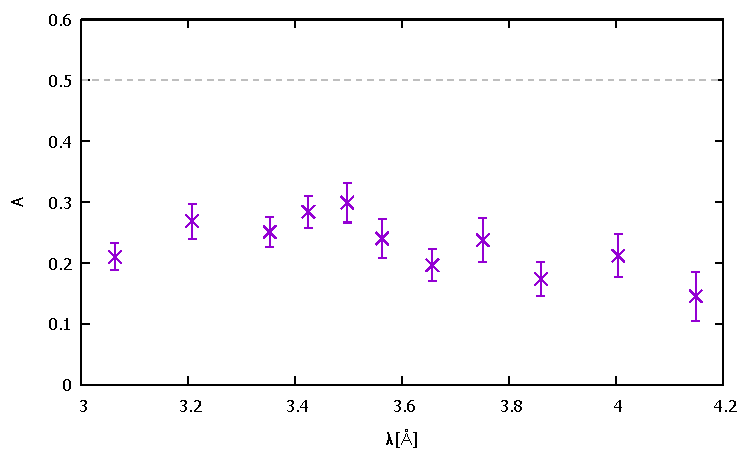
\includegraphics[width=10cm]{discussion/A/A_F.pdf}
\caption{中心波長$\lambda$と$A$の関係} \label{Discussion_fig_A}
\end{minipage}
\end{figure}

\paragraph{解析}
パラメータ$C$に対する考察の結果から$\epsilon/\omega_z=0.131$としたときの$A$の理論値を実験値と共に図\ref{Discussion_fig_A_N4}に表す。このときreduced$\chi^2=1041/12=87$となり、理論値と実験値の一致は悪い。全ての波長において実験値は理論値よりも大きく下にずれている。これは干渉波の振幅が理論の予想より小さいことを意味する。この原因として、バックグラウンドによって波の高さの振動中心が上へずれたことと、位相のずれた波が重ね合わさり振幅が減衰したことの2つが考えられる。
\begin{figure}[h]
\centering
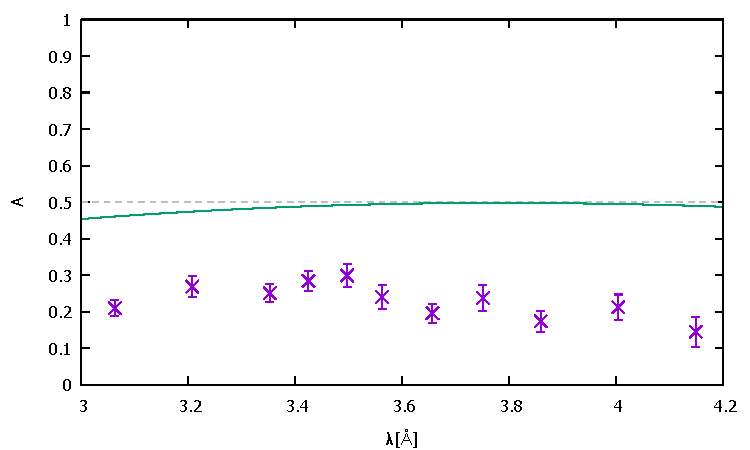
\includegraphics[width=10cm]{discussion/A/A_F_N4.pdf}
\caption{波長に対する$D$の実験値と$\epsilon/\omega_z=0.131$のときの理論値}
\end{figure}

\paragraph{結論}
パラメータ$A$は干渉波の振幅を表し、波の高さと位相の両方に依存する。干渉をみる波長領域の中心波長に対する理論値と実験値は一致せず、実験値は理論値の半分程度となった。観測粒子数にあるバックグラウンドが含まれており、粒子数の変動の中心が数の多い方へずれたこと、実験で得られたデータはある波長領域について観測粒子数を積分したものであり、位相のずれた波が重ね合わさることで振幅が減衰したことが原因として考えられる。

\subsection{中心波長で考えてよい理由}
実験で得られたデータはある波長領域について積分したものであるため、ひとつの波長に対して定められた理論式(\ref{Discussion_theory_ippan})とは厳密には対応づかない。しかし十分狭い波長領域で見れば、近似的に領域の中心の波長に対する理論式とその波長領域での実験値を対応づけることができる。

例えば中心波長$\lambda=3.42$\AA に対して$\pm 0.4$\AA の波長領域を考えると、中心波長における干渉パターンと波長領域で積分したときの干渉パターンは次の図\ref{Discussion_fig_CenterOrInteg1}のようになる。位相シフタコイルに流す電流が増えるにつれ、2つの波が位相についても振幅についてもずれていくのがわかる。
\begin{figure}[h]
\centering
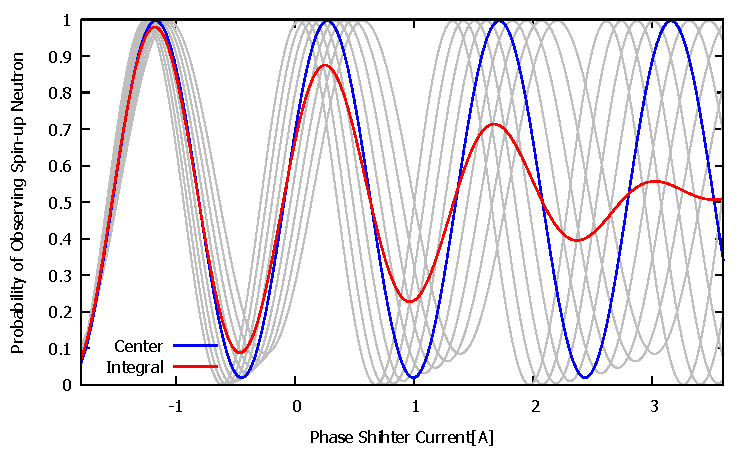
\includegraphics[width=10cm]{discussion/COI/CenterOrInteg1.pdf}
\caption{$\lambda=3.42\pm0.4$\AA のときの中心波長での干渉パターンと干渉パターンの波長領域での積分}\label{Discussion_fig_CenterOrInteg1}
\vspace{-5mm}
\end{figure}

次に十分狭い波長領域$\lambda=3.42\pm0.07$\AA を考え、同様に中心波長における干渉パターンと波長領域で積分したときの干渉パターンを図\ref{Discussion_fig_CenterOrInteg2}に表す。このように、実験を行った電流範囲で見る限り、2つの波の位相はほぼずれず、振幅についてもずれは最大で4\% 程度である。
\begin{figure}[H]
\centering
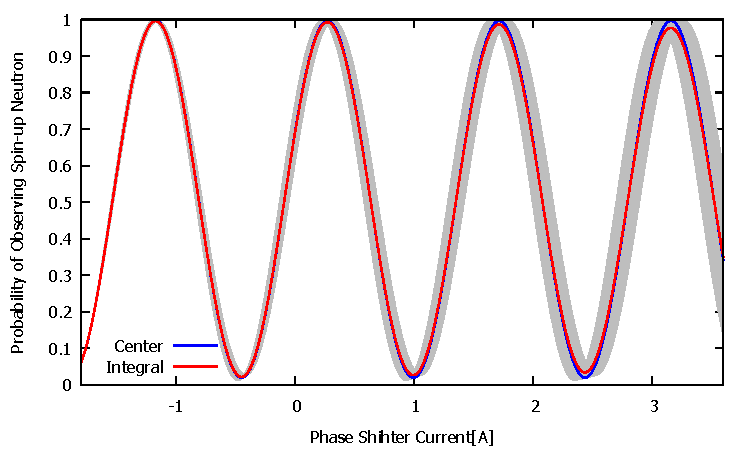
\includegraphics[width=10cm]{discussion/COI/CenterOrInteg2.pdf}
\caption{$\lambda=3.42\pm0.07$\AA のときの中心波長での干渉パターンと干渉パターンの波長領域での積分}\label{Discussion_fig_CenterOrInteg2}
\end{figure}

従って、$\pm0.07$\AA 程度の十分狭い波長領域でみる限り、領域の中心波長に対する理論式とその波長領域での実験値を対応づけることができる。






\section{考察}
前章では干渉パターンを4つの要素に分解し、位相に関係した2つのパラメータ$B,C$については実験結果を理論がよく説明することを見た。しかし波の水深に関係した2つのパラメータ$A,D$については実験結果と理論との間に相違が見られた。この章ではこの相違を説明するために2つの異なる仮説を立て、それぞれ仮説の下で実験結果がうまく説明できるかを考察する。

\subsection{バックグラウンド}
干渉を見る波長領域の中にミラーで反射されていない中性子が混ざっていたとすると、その分干渉波の振動中心は粒子数の多い方にずれ、観測確率として見たときの干渉波の振幅は小さくなることが予想される。

\paragraph{形}
バックグラウンドの分布としてどのような形を仮定するべきか検討を行う。次の図\ref{Discussion2_fig_flipperoff}はスピンフリッパーをOFFにしたときの規格化粒子数の波長分布である。0\AA 付近に高速中性子の立ち上がりが、3.2\AA 付近に反射中性子のピークが見える。そしてその間1\AA 付近にもピークが確認できる。図\ref{Discussion_fig_mirroroff}はミラーを置かずに測定を行ったときの検出粒子数の波長分布であり、1\AA 付近のピークはKUANSからの熱中性子のピークである。すなわち図\ref{Discussion2_fig_flipperoff}の1\AA 付近のピークはミラーで反射されずに検出された熱中性子の一部であると考えられる。
\begin{figure}[H]
%\begin{minipage}{0.5\hsize}
\centering
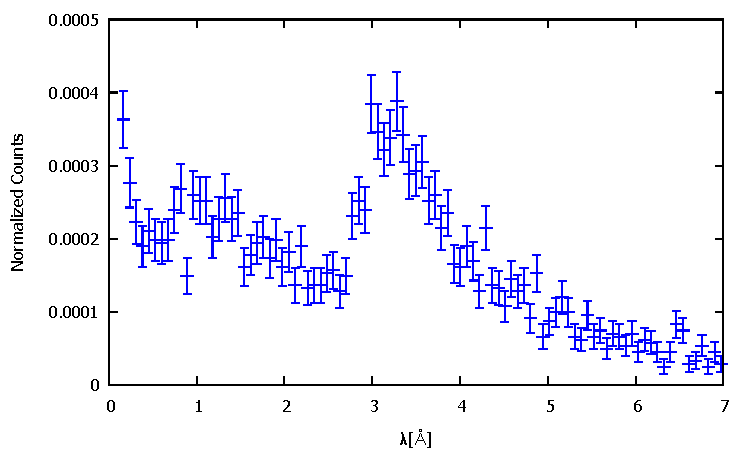
\includegraphics[width=9cm]{discussion/BG/flipperoff.pdf}
\caption{フリッパーOFF時の規格化粒子数波長分布(\ce{^3He}比例計数管による測定)}\label{Discussion2_fig_flipperoff}
%\end{minipage}
%\begin{minipage}{0.5\hsize}
%\centering
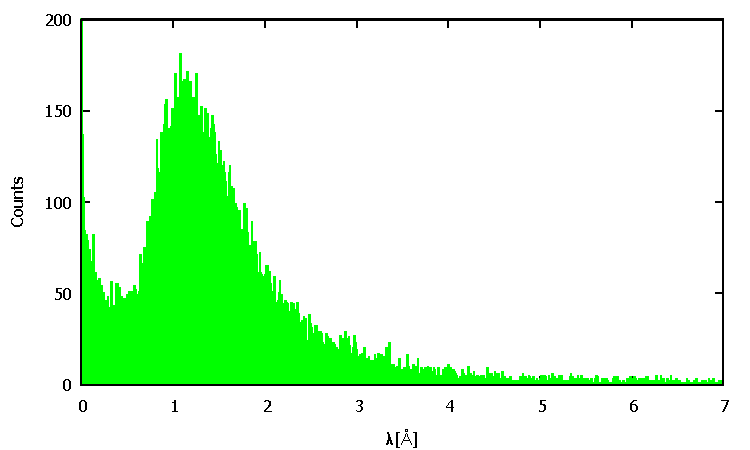
\includegraphics[width=9cm]{discussion/BG/mirroroff.pdf}
\caption{ミラーを置かずに測定した粒子数波長分布(RPMT検出器による測定)}\label{Discussion2_fig_flipperoff}
%\end{minipage}
\end{figure}

次の図\ref{Discussion2_fig_detectormove}はスピンフリッパーOFF時に検出器の$y$座標を、図\ref{Discussion2_fig_flipperoff}の測定位置を$y=0$として、$y=-18,-9,0,+9,+18$mmと動かしたときの規格化粒子数波長分布である。図\ref{Discussion2_fig_detectormove}から$y=0$に近づくにつれ反射中性子のピークが大きくなっていくことがわかるが、5.5\AA 以上の長波長における分布は検出器の位置を動かしてもほとんど一定である。すなわち5.5\AA 以上の長波長においても消えない一定数のバックグラウンドが存在する。
\begin{figure}[h]
\begin{minipage}{0.5\hsize}
\centering
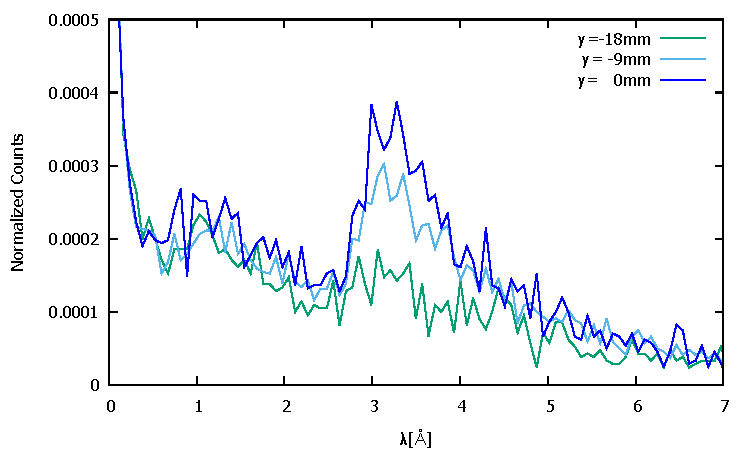
\includegraphics[width=\hsize]{discussion/BG/flippermove1.pdf}
\end{minipage}
\begin{minipage}{0.5\hsize}
\centering
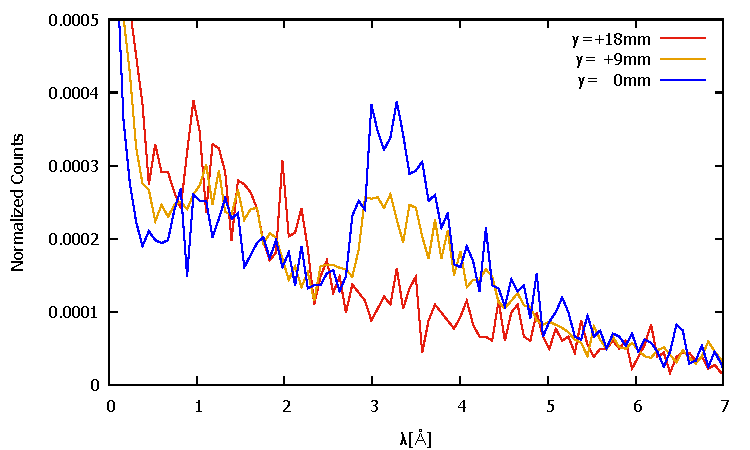
\includegraphics[width=\hsize]{discussion/BG/flippermove2.pdf}
\end{minipage}
\caption{検出器の位置を動かしたときの規格化粒子数}\label{Discussion2_fig_detectormove}
\end{figure}

以上からバックグラウンドとしてあるピークを持ち長波長で消えないものを取りたい。そこで最もシンプルにガウシアンに定数項のついた$a\exp(-(x-b)^2/2c^2)+d$の形を採用する。なおもともとの熱中性子はMaxwell分布に従うが、バックグラウンドとして検出されたものは壁などで反射された成分などを含み元の分布とは異なると考えられるため、シンプルな形を採用した。図\ref{Discussion2_fig_flipperoff}を反射成分を除く0.5-2.5と5.5-7\AA の範囲でフィッティングした結果を図\ref{Discussion2_fig_backfit}に表し、各パラメータの値を表\ref{Discussion2_tbl_backfit}に示す。

\begin{figure}[H]
\begin{minipage}{0.7\hsize}
\centering
%\vspace{2.5cm}
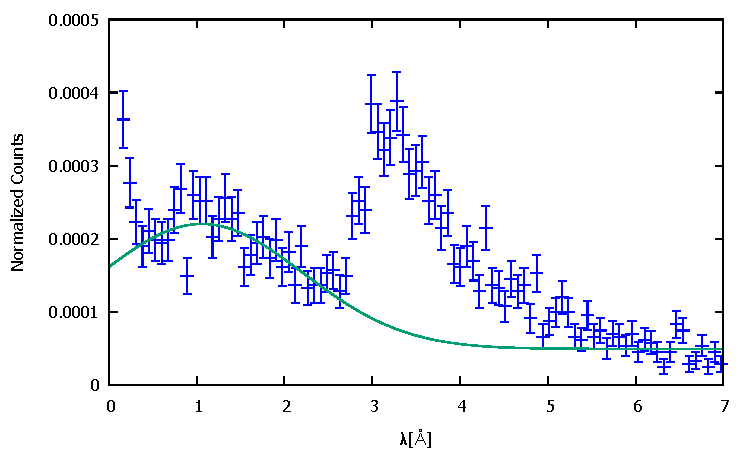
\includegraphics[width=10cm]{discussion/BG/background.pdf}
\caption{バックグラウンド} \label{Discussion2_fig_backfit}
\end{minipage}
\begin{minipage}{0.3\hsize}
\centering
\makeatletter
\def\@captype{table}
\makeatother
\caption{各パラメータ} \label{Discussion2_tbl_backfit}
\begin{tabular}{|c|c|} \hline
$a$&$1.7\times 10^{-4}\pm 1\times10^{-5}$\\ \hline
$b$&$1.1\pm0.2$\\ \hline
$c$&$1.1\pm0.2$\\ \hline
$d$&$4.9\times 10^{-5}\pm4\times 10^{-6}$\\ \hline
\end{tabular}
\end{minipage}
\end{figure}

\paragraph{結果}
章と同様に次の手順でバックグラウンドを考慮した場合のスピン上向き中性子観測確率の干渉パターンとフィッティングパラメータ$A,B,C,D$を得た。
\begin{enumerate}
\item シフタコイル電流を変えていったときの規格化粒子数の波長分布(図\ref{Discussion2_fig_NC})からバックグラウンドを取り除いた分布(図\ref{Discussion2_fig_NC_b})を得た
\item 図\ref{Discussion2_fig_NC_b}の分布において種々の中心波長$\pm0.07$\AA の波長領域に含まれる規格化粒子数を数え、シフタコイル電流を横軸とした干渉パターン(図\ref{Discussion2_fig_IF_nb})を得た
\item 干渉パターンを$-A'\cos(Bx+C)+D'$でフィットした
\item フリッパーOFF時の規格化粒子数からバックグラウンドを除いた分布から、そろぞれの波長領域における干渉パターンの縦軸(規格化粒子数)をスピン上向き中性子の観測確率とするためのファクターを求めた
\item 図\ref{Discussion2_fig_IF_nb}を上で求めたファクターで割り、スピン上向き中性子の観測確率の干渉パターン(図\ref{Discussion2_fig_IF_rb})を得た
\item フィッティングパラメータ$A',D'$をファクターで割り、理論と比較可能なパラメータ$A,B,C,D$を得た(表\ref{Discussion2_tbl_IF_rb})
\end{enumerate}

\begin{figure}[h]
\begin{minipage}{0.33\hsize}
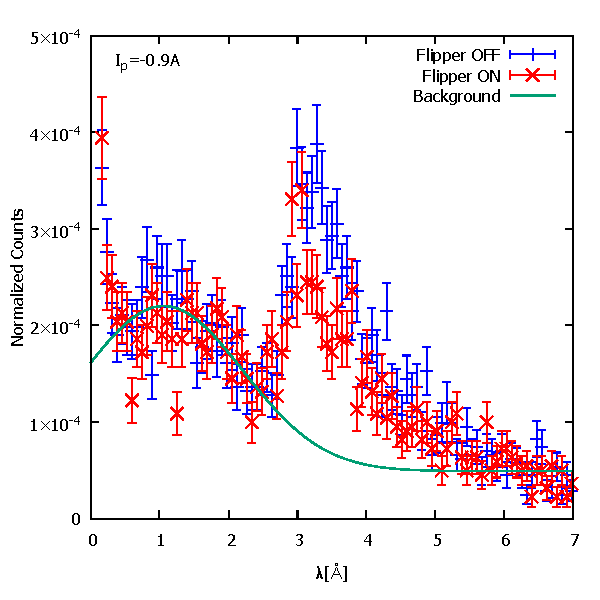
\includegraphics[width=5cm]{discussion/NC/NormalizedCounts_-9A.pdf}
\end{minipage}
\begin{minipage}{0.33\hsize}
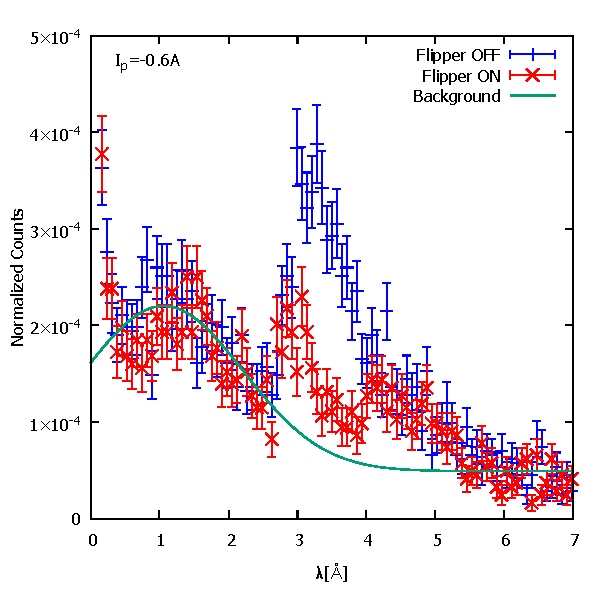
\includegraphics[width=5cm]{discussion/NC/NormalizedCounts_-6A.pdf}
\end{minipage}
\begin{minipage}{0.33\hsize}
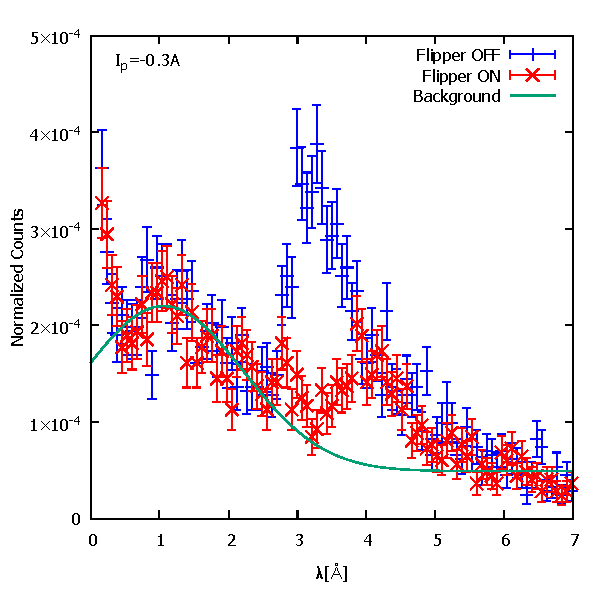
\includegraphics[width=5cm]{discussion/NC/NormalizedCounts_-3A.pdf}
\end{minipage}\\
\begin{minipage}{0.33\hsize}
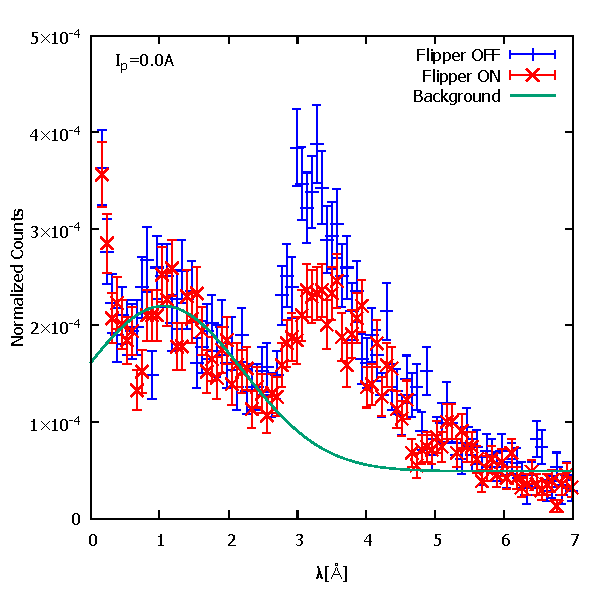
\includegraphics[width=5cm]{discussion/NC/NormalizedCounts_0A.pdf}
\end{minipage}
\begin{minipage}{0.33\hsize}
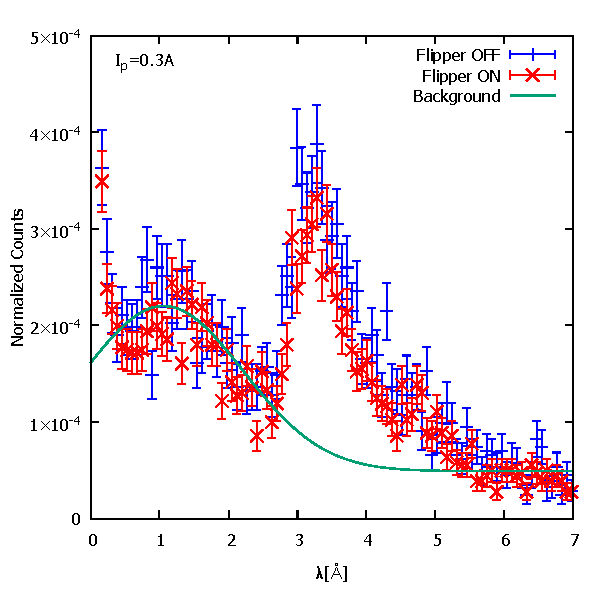
\includegraphics[width=5cm]{discussion/NC/NormalizedCounts_3A.pdf}
\end{minipage}
\begin{minipage}{0.33\hsize}
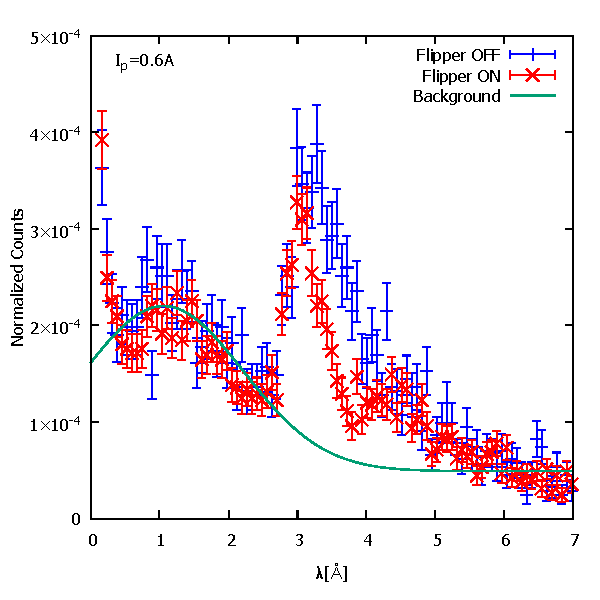
\includegraphics[width=5cm]{discussion/NC/NormalizedCounts_6A.pdf}
\end{minipage}\\
\begin{minipage}{0.33\hsize}
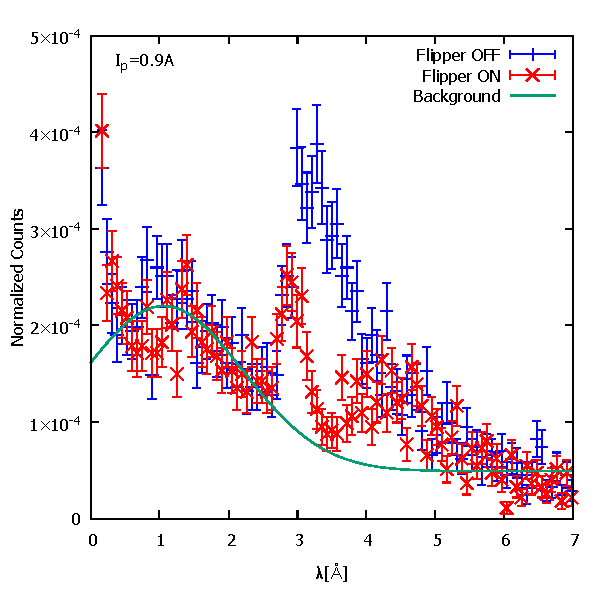
\includegraphics[width=5cm]{discussion/NC/NormalizedCounts_9A.pdf}
\end{minipage}
\begin{minipage}{0.33\hsize}
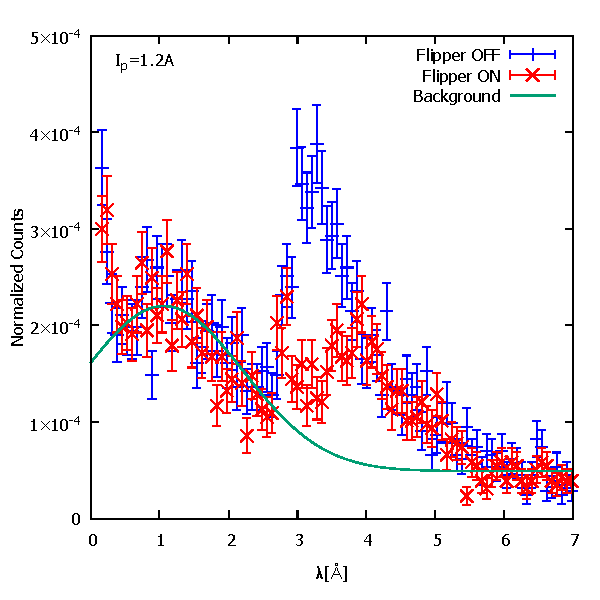
\includegraphics[width=5cm]{discussion/NC/NormalizedCounts_12A.pdf}
\end{minipage}
\begin{minipage}{0.33\hsize}
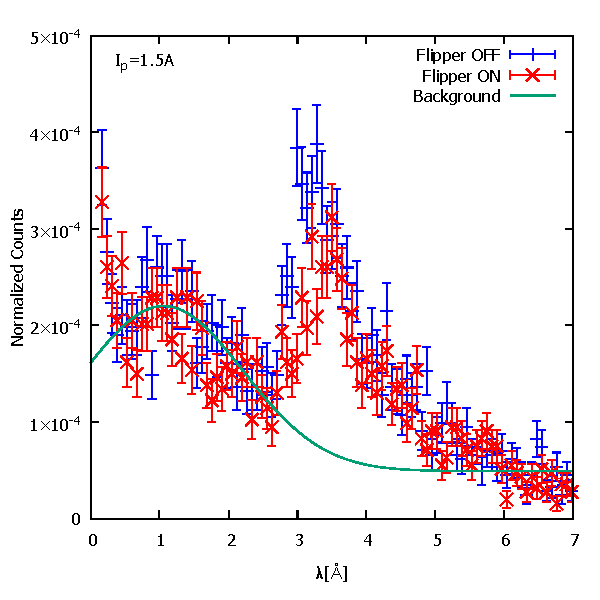
\includegraphics[width=5cm]{discussion/NC/NormalizedCounts_15A.pdf}
\end{minipage}\\
\begin{minipage}{0.33\hsize}
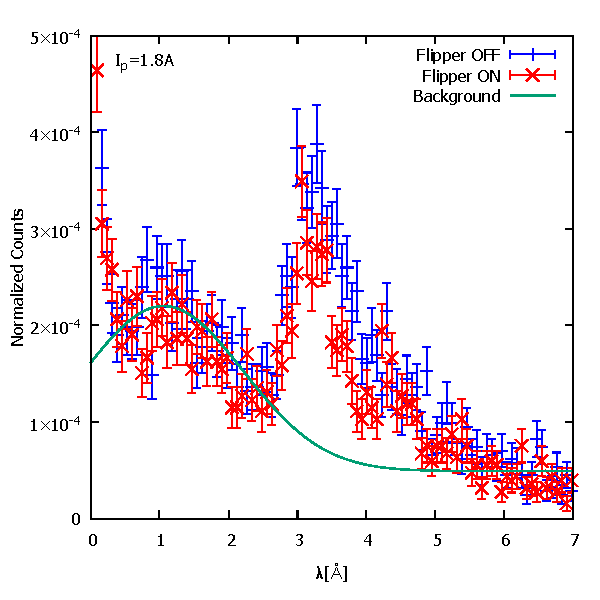
\includegraphics[width=5cm]{discussion/NC/NormalizedCounts_18A.pdf}
\end{minipage}
\begin{minipage}{0.33\hsize}
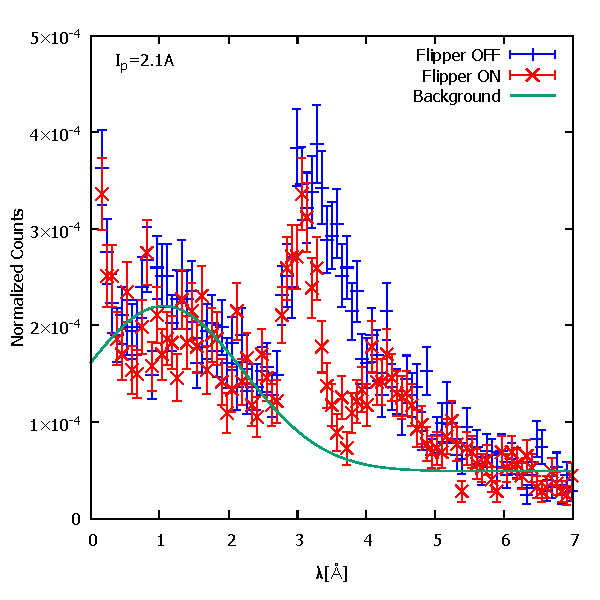
\includegraphics[width=5cm]{discussion/NC/NormalizedCounts_21A.pdf}
\end{minipage}
\begin{minipage}{0.33\hsize}
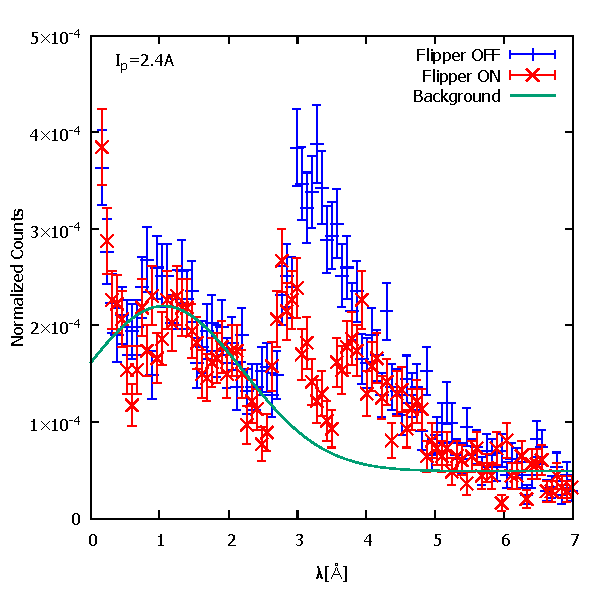
\includegraphics[width=5cm]{discussion/NC/NormalizedCounts_24A.pdf}
\end{minipage}
\caption{規格化粒子数の波長分布(バックグラウンドを引く前)}\label{Discussion2_fig_NC}
\end{figure}

\begin{figure}[h]
\begin{minipage}{0.33\hsize}
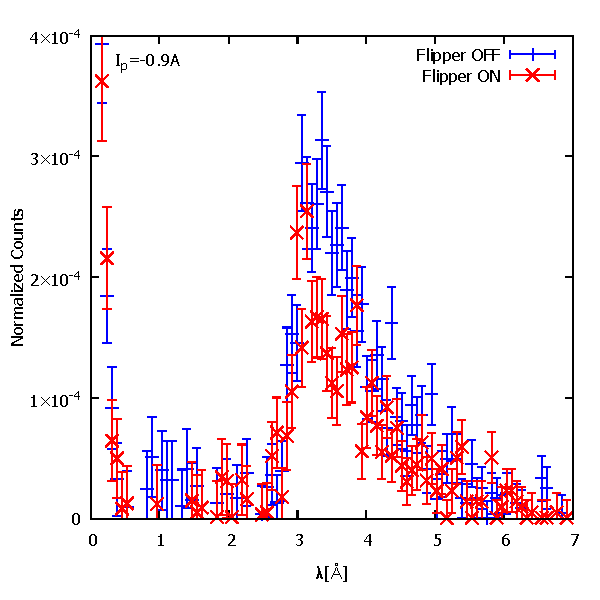
\includegraphics[width=5cm]{discussion/NC-BG/NormalizedCounts_b_-9A.pdf}
\end{minipage}
\begin{minipage}{0.33\hsize}
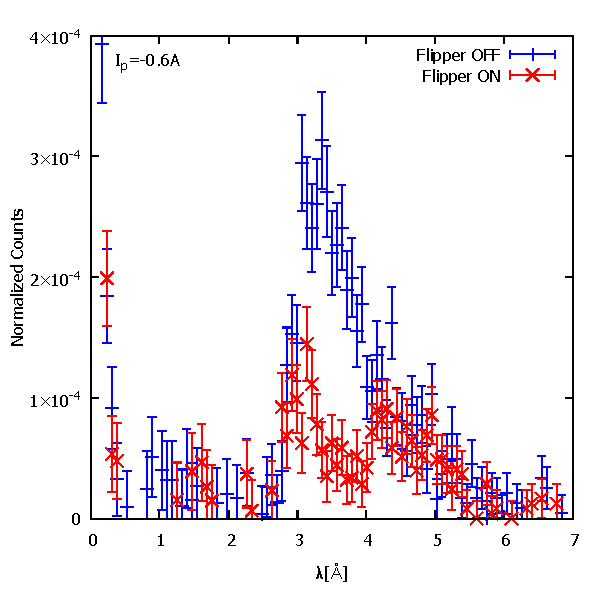
\includegraphics[width=5cm]{discussion/NC-BG/NormalizedCounts_b_-6A.pdf}
\end{minipage}
\begin{minipage}{0.33\hsize}
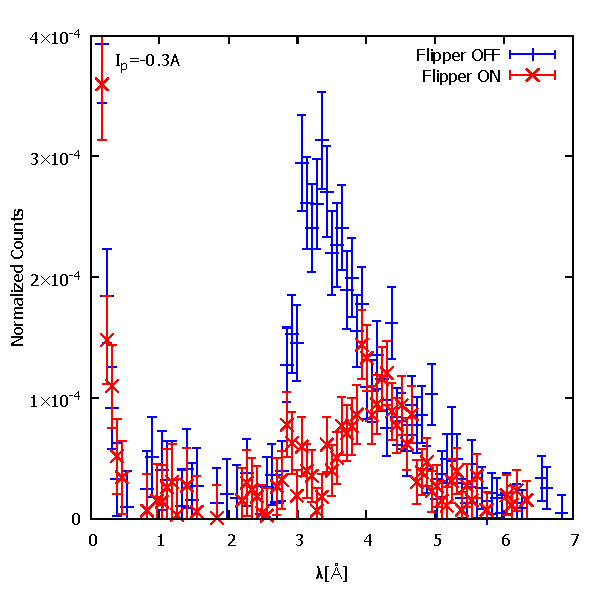
\includegraphics[width=5cm]{discussion/NC-BG/NormalizedCounts_b_-3A.pdf}
\end{minipage}\\
\begin{minipage}{0.33\hsize}
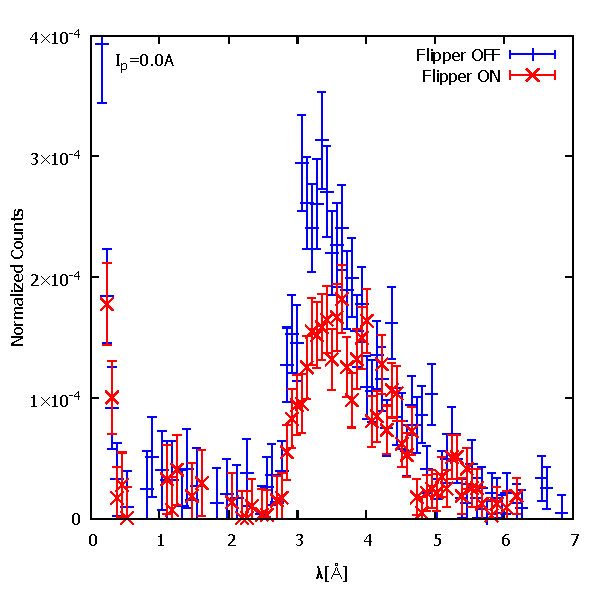
\includegraphics[width=5cm]{discussion/NC-BG/NormalizedCounts_b_0A.pdf}
\end{minipage}
\begin{minipage}{0.33\hsize}
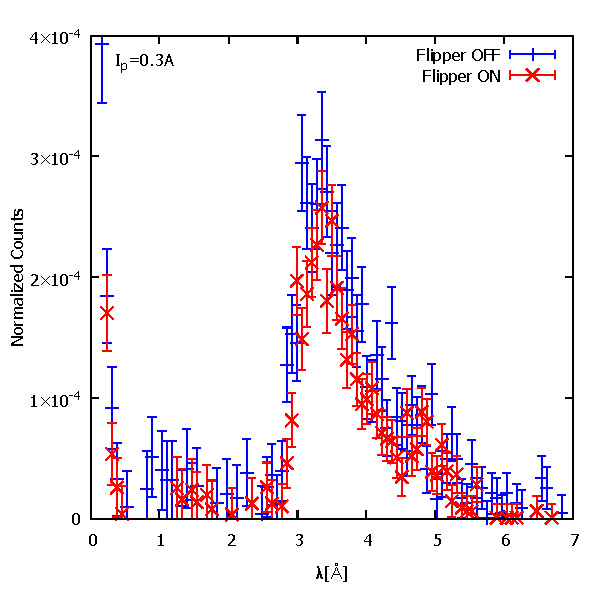
\includegraphics[width=5cm]{discussion/NC-BG/NormalizedCounts_b_3A.pdf}
\end{minipage}
\begin{minipage}{0.33\hsize}
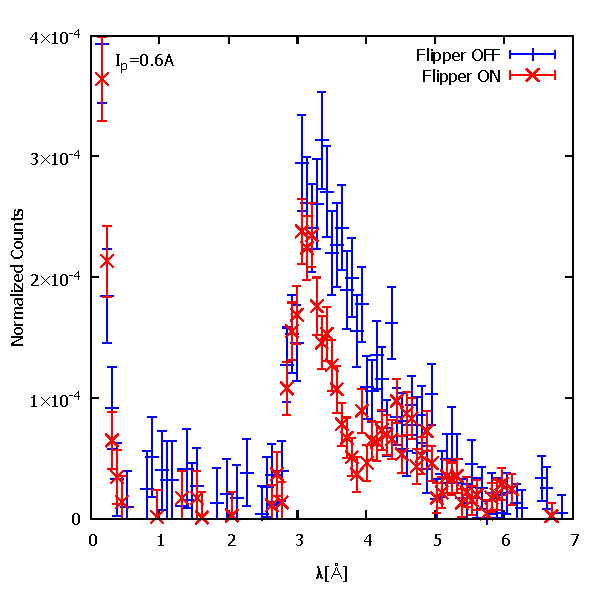
\includegraphics[width=5cm]{discussion/NC-BG/NormalizedCounts_b_6A.pdf}
\end{minipage}\\
\begin{minipage}{0.33\hsize}
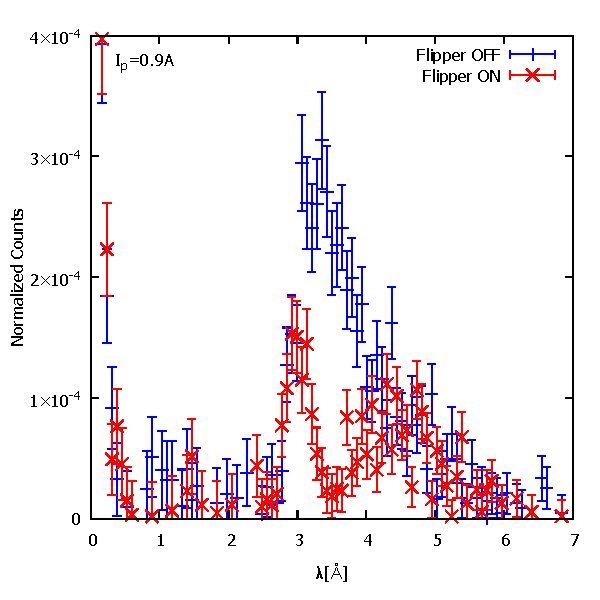
\includegraphics[width=5cm]{discussion/NC-BG/NormalizedCounts_b_9A.pdf}
\end{minipage}
\begin{minipage}{0.33\hsize}
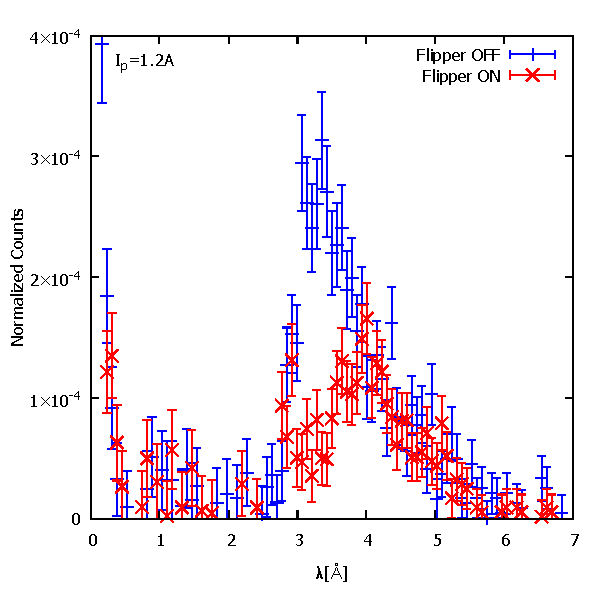
\includegraphics[width=5cm]{discussion/NC-BG/NormalizedCounts_b_12A.pdf}
\end{minipage}
\begin{minipage}{0.33\hsize}
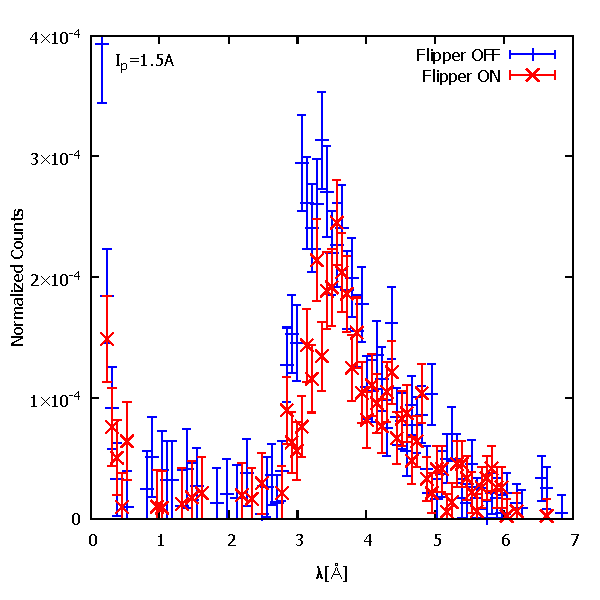
\includegraphics[width=5cm]{discussion/NC-BG/NormalizedCounts_b_15A.pdf}
\end{minipage}\\
\begin{minipage}{0.33\hsize}
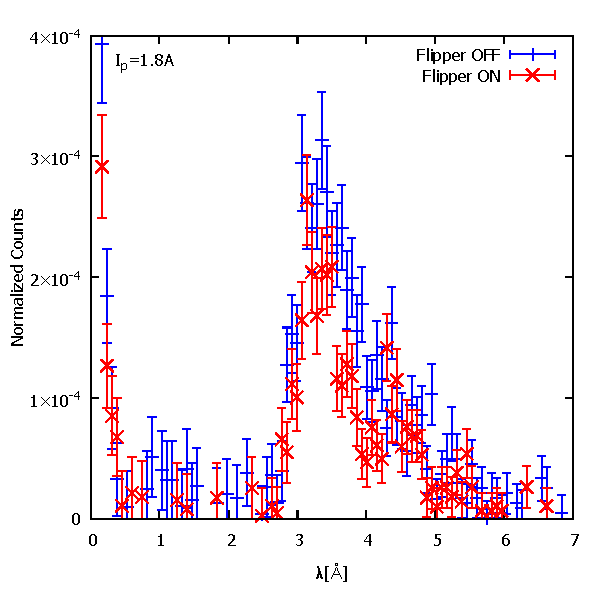
\includegraphics[width=5cm]{discussion/NC-BG/NormalizedCounts_b_18A.pdf}
\end{minipage}
\begin{minipage}{0.33\hsize}
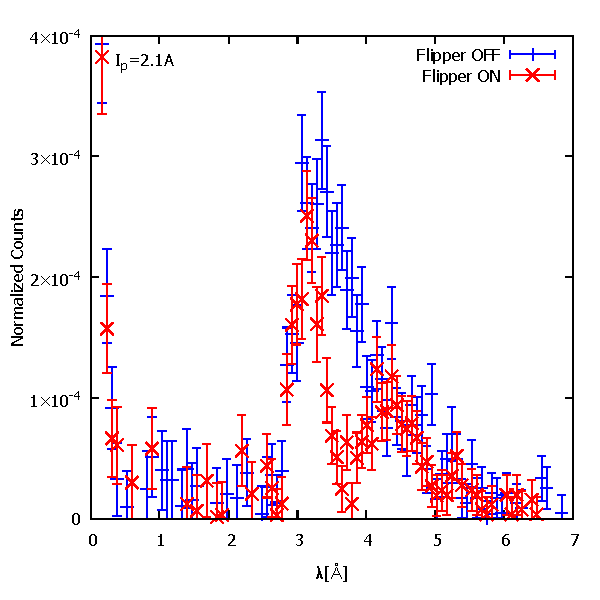
\includegraphics[width=5cm]{discussion/NC-BG/NormalizedCounts_b_21A.pdf}
\end{minipage}
\begin{minipage}{0.33\hsize}
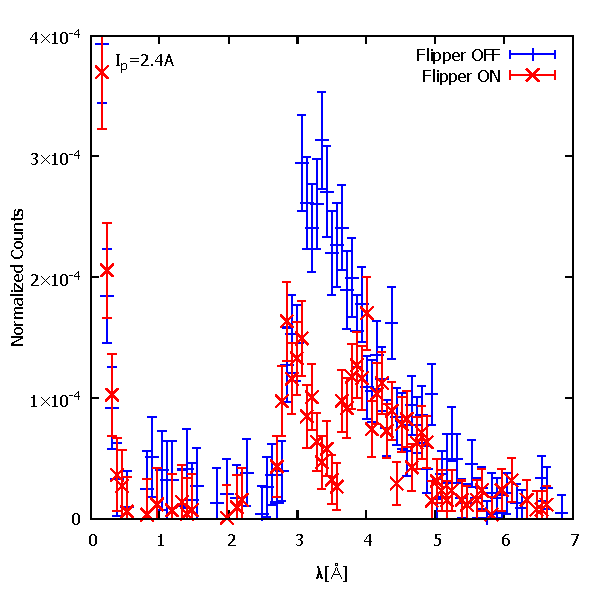
\includegraphics[width=5cm]{discussion/NC-BG/NormalizedCounts_b_24A.pdf}
\end{minipage}
\caption{規格化粒子数の波長分布(バックグラウンドを引いた後)}\label{Discussion2_fig_NC_b}
\end{figure}

\begin{figure}[h]
\begin{minipage}{0.33\hsize}
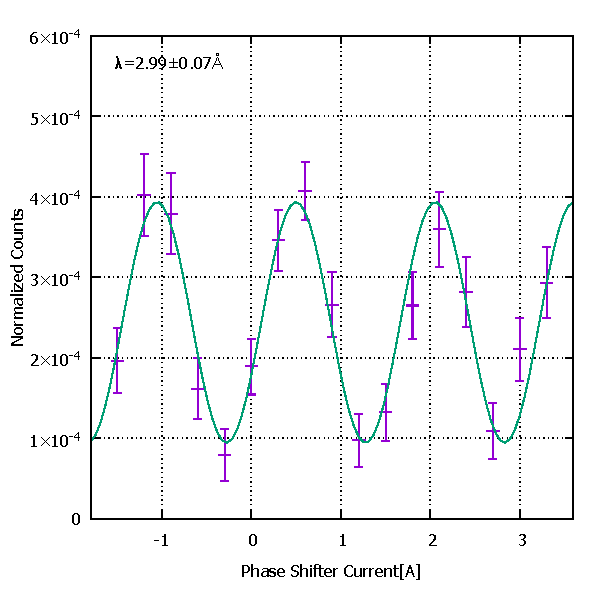
\includegraphics[width=5cm]{discussion/IF_nb/Interference_nb_fit420.pdf}
\end{minipage}
\begin{minipage}{0.33\hsize}
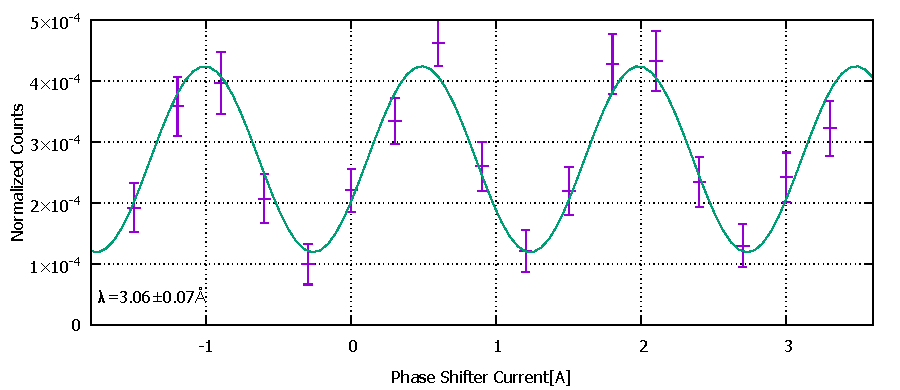
\includegraphics[width=5cm]{discussion/IF_nb/Interference_nb_fit430.pdf}
\end{minipage}
\begin{minipage}{0.33\hsize}
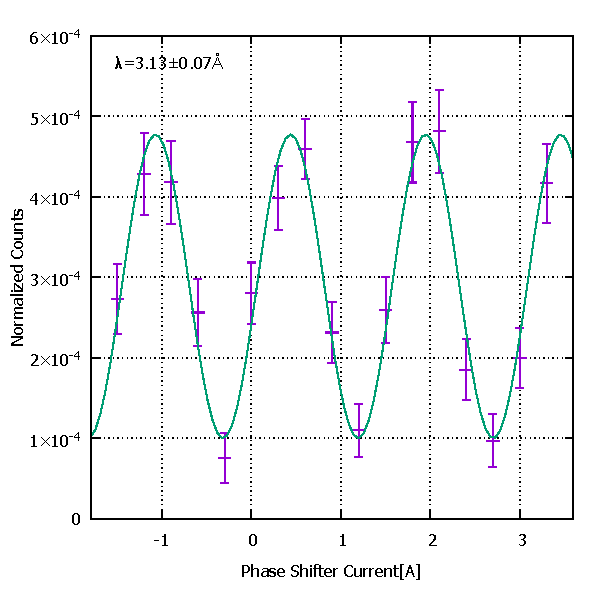
\includegraphics[width=5cm]{discussion/IF_nb/Interference_nb_fit440.pdf}
\end{minipage}\\
\begin{minipage}{0.33\hsize}
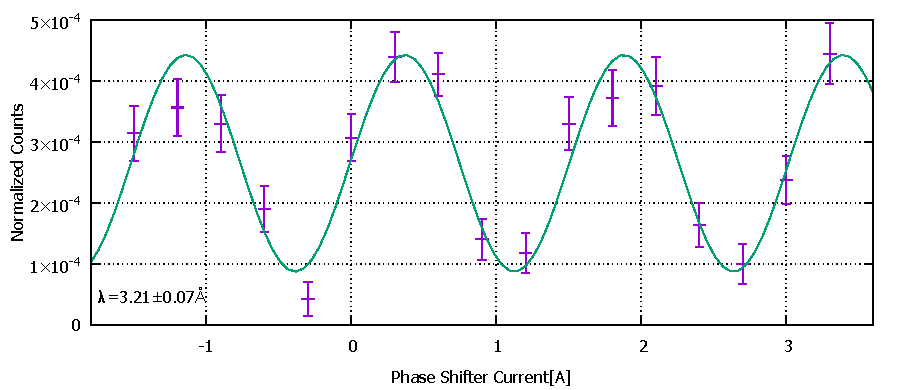
\includegraphics[width=5cm]{discussion/IF_nb/Interference_nb_fit450.pdf}
\end{minipage}
\begin{minipage}{0.33\hsize}
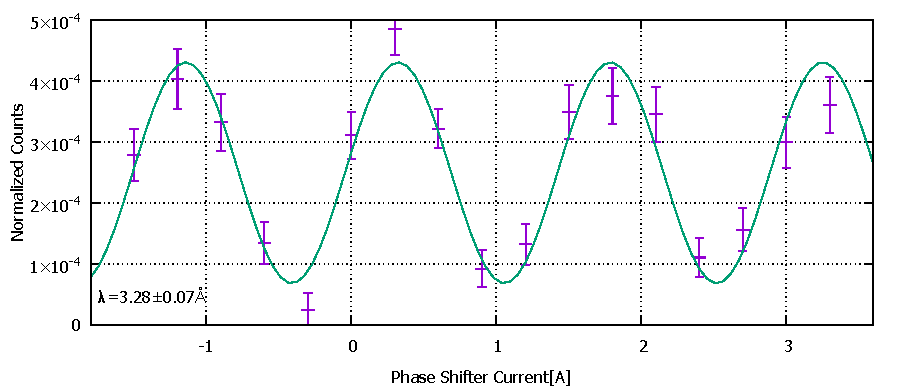
\includegraphics[width=5cm]{discussion/IF_nb/Interference_nb_fit460.pdf}
\end{minipage}
\begin{minipage}{0.33\hsize}
\includegraphics[width=5cm]{discussion/IF_nb/Interference_nb_fit470.pdf}
\end{minipage}\\
\begin{minipage}{0.33\hsize}
\includegraphics[width=5cm]{discussion/IF_nb/Interference_nb_fit480.pdf}
\end{minipage}
\begin{minipage}{0.33\hsize}
\includegraphics[width=5cm]{discussion/IF_nb/Interference_nb_fit490.pdf}
\end{minipage}
\begin{minipage}{0.33\hsize}
\includegraphics[width=5cm]{discussion/IF_nb/Interference_nb_fit500.pdf}
\end{minipage}\\
\begin{minipage}{0.33\hsize}
\includegraphics[width=5cm]{discussion/IF_nb/Interference_nb_fit510.pdf}
\end{minipage}
\begin{minipage}{0.33\hsize}
\includegraphics[width=5cm]{discussion/IF_nb/Interference_nb_fit520.pdf}
\end{minipage}
\begin{minipage}{0.33\hsize}
\includegraphics[width=5cm]{discussion/IF_nb/Interference_nb_fit530.pdf}
\end{minipage}
\caption{規格化粒子数の干渉パターン}\label{Discussion2_fig_IF_nb}
\end{figure}

\begin{figure}[h]
\begin{minipage}{0.33\hsize}
\includegraphics[width=5cm]{discussion/IF_rb/Interference_rb_fit420.pdf}
\end{minipage}
\begin{minipage}{0.33\hsize}
\includegraphics[width=5cm]{discussion/IF_rb/Interference_rb_fit430.pdf}
\end{minipage}
\begin{minipage}{0.33\hsize}
\includegraphics[width=5cm]{discussion/IF_rb/Interference_rb_fit440.pdf}
\end{minipage}\\
\begin{minipage}{0.33\hsize}
\includegraphics[width=5cm]{discussion/IF_rb/Interference_rb_fit450.pdf}
\end{minipage}
\begin{minipage}{0.33\hsize}
\includegraphics[width=5cm]{discussion/IF_rb/Interference_rb_fit460.pdf}
\end{minipage}
\begin{minipage}{0.33\hsize}
\includegraphics[width=5cm]{discussion/IF_rb/Interference_rb_fit470.pdf}
\end{minipage}\\
\begin{minipage}{0.33\hsize}
\includegraphics[width=5cm]{discussion/IF_rb/Interference_rb_fit480.pdf}
\end{minipage}
\begin{minipage}{0.33\hsize}
\includegraphics[width=5cm]{discussion/IF_rb/Interference_rb_fit490.pdf}
\end{minipage}
\begin{minipage}{0.33\hsize}
\includegraphics[width=5cm]{discussion/IF_rb/Interference_rb_fit500.pdf}
\end{minipage}\\
\begin{minipage}{0.33\hsize}
\includegraphics[width=5cm]{discussion/IF_rb/Interference_rb_fit510.pdf}
\end{minipage}
\begin{minipage}{0.33\hsize}
\includegraphics[width=5cm]{discussion/IF_rb/Interference_rb_fit520.pdf}
\end{minipage}
\begin{minipage}{0.33\hsize}
\includegraphics[width=5cm]{discussion/IF_rb/Interference_rb_fit530.pdf}
\end{minipage}
\caption{スピン上向き中性子観測確率の干渉パターン}\label{Discussion2_fig_IF_rb}
\end{figure}

\clearpage
\begin{table}[h]
\centering
\caption{各中心波長$\lambda$に対するパラメータ$A,B,C,D$とreduced$\chi^2$}
\begin{tabular}{cccccc}
$\lambda$[\AA]&$A$&$B$&$C$&$D$&reduced$\chi^2$\\ \hline
2.92 	&	0.36 	$\pm$	0.07 	&	3.84 	$\pm$	0.07 	&	0.92 	$\pm$	0.13 	&	0.76 	$\pm$	0.12 	&	0.78 	\\
2.99 	&	0.34 	$\pm$	0.05 	&	4.04 	$\pm$	0.05 	&	1.13 	$\pm$	0.09 	&	0.55 	$\pm$	0.07 	&	0.80 	\\
3.06 	&	0.27 	$\pm$	0.03 	&	4.20 	$\pm$	0.05 	&	1.11 	$\pm$	0.09 	&	0.49 	$\pm$	0.05 	&	0.75 	\\
3.13 	&	0.38 	$\pm$	0.05 	&	4.16 	$\pm$	0.04 	&	1.32 	$\pm$	0.07 	&	0.58 	$\pm$	0.06 	&	0.66 	\\
3.21 	&	0.36 	$\pm$	0.05 	&	4.16 	$\pm$	0.06 	&	1.61 	$\pm$	0.10 	&	0.53 	$\pm$	0.06 	&	1.26 	\\
3.28 	&	0.32 	$\pm$	0.04 	&	4.29 	$\pm$	0.06 	&	1.76 	$\pm$	0.10 	&	0.43 	$\pm$	0.05 	&	1.33 	\\
3.35 	&	0.31 	$\pm$	0.03 	&	4.29 	$\pm$	0.04 	&	1.89 	$\pm$	0.06 	&	0.42 	$\pm$	0.04 	&	0.58 	\\
3.42 	&	0.37 	$\pm$	0.04 	&	4.41 	$\pm$	0.04 	&	2.03 	$\pm$	0.06 	&	0.49 	$\pm$	0.05 	&	0.58 	\\
3.50 	&	0.39 	$\pm$	0.05 	&	4.52 	$\pm$	0.04 	&	2.13 	$\pm$	0.07 	&	0.51 	$\pm$	0.06 	&	0.80 	\\
3.57 	&	0.31 	$\pm$	0.05 	&	4.63 	$\pm$	0.07 	&	2.31 	$\pm$	0.11 	&	0.47 	$\pm$	0.05 	&	1.39 	\\
3.64 	&	0.27 	$\pm$	0.04 	&	4.76 	$\pm$	0.06 	&	2.45 	$\pm$	0.10 	&	0.49 	$\pm$	0.06 	&	0.70 	\\
3.71 	&	0.28 	$\pm$	0.05 	&	4.74 	$\pm$	0.09 	&	2.56 	$\pm$	0.15 	&	0.50 	$\pm$	0.06 	&	1.30 	\\
3.79 	&	0.29 	$\pm$	0.05 	&	4.76 	$\pm$	0.11 	&	2.60 	$\pm$	0.17 	&	0.53 	$\pm$	0.07 	&	1.64 	\\
3.86 	&	0.23 	$\pm$	0.04 	&	5.06 	$\pm$	0.10 	&	2.89 	$\pm$	0.16 	&	0.57 	$\pm$	0.08 	&	0.84 	\\
3.93 	&	0.29 	$\pm$	0.07 	&	5.02 	$\pm$	0.13 	&	3.44 	$\pm$	0.22 	&	0.65 	$\pm$	0.10 	&	1.72 	\\
4.00 	&	0.32 	$\pm$	0.07 	&	5.13 	$\pm$	0.08 	&	3.12 	$\pm$	0.14 	&	0.87 	$\pm$	0.15 	&	0.48 	\\ \hline
\end{tabular}
\end{table}

\paragraph{解析・考察}
バックグラウンドを考慮することによって各パラメータはどのように変わり変わらなかったのか分析を行い、その理由を考察する。
表\ref{Discussion2_tbl_ABCDb}にパラメータ$A,B,C,D$のバックグラウンド考慮前、考慮後の実験値と理論値をそれぞれ示し、その結果を図\ref{Discussion2_fig_ABCDb}に表す。表\ref{Discussion2_tbl_ABCDb}と図\ref{Discussion2_fig_ABCDb}から次のことが考察できる。
\begin{itemize}
\item パラメータ$B,C$は位相に関係した量であるからバックグラウンドによる影響はほぼなく、バックグラウンドを考慮する前と後で有効数字の範囲では誤差も含めて全く変化しない。したがって実験値と理論値はよく一致したまま保たれる。
\item パラメータ$D$は波の水深に関係する量であるからバックグラウンドの影響を受ける。バックグラウンドを考慮すると全体に小さくなる方へシフトし、3.0-3.8\AA の領域では実験値と理論値はよく一致する。領域の外では実験値が理論値よりも上へとずれてゆく。これは波長3\AA 以下や4\AA 以上では反射中性子の数が少なくなるため、下で述べるような粒子数を変化させる他の要因に強く影響されるためと考えられる。
\item パラメータ$A$も$D$と同じく波の水深に関係する量であるからバックグラウンドの影響を受ける。バックグラウンドを考慮すると、理論で予想されるまでには届かないものの、全体に上へシフトする。パラメータ$A$は位相の影響も受け、$\pm 0.07$\AA の波長領域で積分すると理論値は最大4\% 程度小さくなることを考慮すれば、理論値と実験値はさらに近づく。このようにパラメータ$A$は様々な影響を複合的に受けるためずれの原因をつきとめるのは困難であるが、次に述べるような粒子数を変化させる他の要因にも大きく影響されると考えられる。
\item 粒子数を変化させる他の要因としては、不均一磁場による軌道の変化や、空気によるスピンの反転、地磁気などの外部磁場によるスピンの反転などが考えられるが定量的な議論は難しい。
\end{itemize}

\begin{table}[H]
\caption{バックグラウンド考慮前後における実験値と理論値}\label{Discussion2_tbl_ABCDb}
\begin{minipage}{0.5\hsize}
\subcaption{$A$}
\centering
\begin{tabular}{cccc}
$\lambda$[\AA]&BG考慮前&BG考慮後&理論値\\ \hline
2.92&0.21$\pm$0.03&0.36$\pm$0.07&0.44\\
2.99 	&	0.24 	$\pm$	0.03 	&	0.34 	$\pm$	0.05 	&	0.45 	\\
3.06 	&	0.21 	$\pm$	0.02 	&	0.27 	$\pm$	0.03 	&	0.46 	\\
3.13 	&	0.28 	$\pm$	0.03 	&	0.38 	$\pm$	0.05 	&	0.47 	\\
3.21 	&	0.27 	$\pm$	0.03 	&	0.36 	$\pm$	0.05 	&	0.47 	\\
3.28 	&	0.25 	$\pm$	0.03 	&	0.32 	$\pm$	0.04 	&	0.48 	\\
3.35 	&	0.25 	$\pm$	0.02 	&	0.31 	$\pm$	0.03 	&	0.48 	\\
3.42 	&	0.29 	$\pm$	0.03 	&	0.37 	$\pm$	0.04 	&	0.49 	\\
3.50 	&	0.30 	$\pm$	0.03 	&	0.39 	$\pm$	0.05 	&	0.49 	\\
3.57 	&	0.24 	$\pm$	0.03 	&	0.31 	$\pm$	0.05 	&	0.49 	\\
3.64 	&	0.21 	$\pm$	0.03 	&	0.27 	$\pm$	0.04 	&	0.50 	\\
3.71 	&	0.21 	$\pm$	0.03 	&	0.28 	$\pm$	0.05 	&	0.50 	\\
3.79 	&	0.22 	$\pm$	0.04 	&	0.29 	$\pm$	0.05 	&	0.50 	\\
3.86 	&	0.17 	$\pm$	0.03 	&	0.23 	$\pm$	0.04 	&	0.50 	\\
3.93 	&	0.21 	$\pm$	0.04 	&	0.29 	$\pm$	0.07 	&	0.50 	\\
4.00 	&	0.21 	$\pm$	0.03 	&	0.32 	$\pm$	0.07 	&	0.50	\\ \hline
\end{tabular}
\vspace{5mm}
\end{minipage}
\begin{minipage}{0.5\hsize}
\subcaption{$B$}
\centering
\begin{tabular}{cccc}
$\lambda$[\AA]&BG考慮前&BG考慮後&理論値\\ \hline
2.92&3.84$\pm$0.07&3.84$\pm$0.07&3.71\\
2.99 	&	4.04 	$\pm$	0.05 	&	4.04 	$\pm$	0.05 	&	3.81 	\\
3.06 	&	4.20 	$\pm$	0.05 	&	4.20 	$\pm$	0.05 	&	3.90 	\\
3.13 	&	4.16 	$\pm$	0.04 	&	4.16 	$\pm$	0.04 	&	3.99 	\\
3.21 	&	4.16 	$\pm$	0.06 	&	4.16 	$\pm$	0.06 	&	4.08 	\\
3.28 	&	4.29 	$\pm$	0.06 	&	4.29 	$\pm$	0.06 	&	4.18 	\\
3.35 	&	4.29 	$\pm$	0.04 	&	4.29 	$\pm$	0.04 	&	4.27 	\\
3.42 	&	4.41 	$\pm$	0.04 	&	4.41 	$\pm$	0.04 	&	4.36 	\\
3.50 	&	4.52 	$\pm$	0.04 	&	4.52 	$\pm$	0.04 	&	4.45 	\\
3.57 	&	4.63 	$\pm$	0.07 	&	4.63 	$\pm$	0.07 	&	4.54 	\\
3.64 	&	4.76 	$\pm$	0.06 	&	4.76 	$\pm$	0.06 	&	4.64 	\\
3.71 	&	4.74 	$\pm$	0.09 	&	4.74 	$\pm$	0.09 	&	4.73 	\\
3.79 	&	4.76 	$\pm$	0.11 	&	4.76 	$\pm$	0.11 	&	4.82 	\\
3.86 	&	5.06 	$\pm$	0.10 	&	5.06 	$\pm$	0.10 	&	4.91 	\\
3.93 	&	5.02 	$\pm$	0.13 	&	5.02 	$\pm$	0.13 	&	5.01 	\\
4.00 	&	5.13 	$\pm$	0.08 	&	5.13 	$\pm$	0.08 	&	5.10 	\\ \hline
\end{tabular}
\vspace{5mm}
\end{minipage}\\
\begin{minipage}{0.5\hsize}
\subcaption{$C$}
\centering
\begin{tabular}{cccc}
$\lambda$[\AA]&BG考慮前&BG考慮後&理論値\\ \hline
2.92&0.92$\pm$0.13&0.92$\pm$0.13&0.71\\
2.99 	&	1.13 	$\pm$	0.09 	&	1.13 	$\pm$	0.09 	&	0.89 	\\
3.06 	&	1.11 	$\pm$	0.09 	&	1.11 	$\pm$	0.09 	&	1.07 	\\
3.13 	&	1.32 	$\pm$	0.07 	&	1.32 	$\pm$	0.07 	&	1.25 	\\
3.21 	&	1.61 	$\pm$	0.10 	&	1.61 	$\pm$	0.10 	&	1.43 	\\
3.28 	&	1.76 	$\pm$	0.10 	&	1.76 	$\pm$	0.10 	&	1.61 	\\
3.35 	&	1.89 	$\pm$	0.06 	&	1.89 	$\pm$	0.06 	&	1.80 	\\
3.42 	&	2.03 	$\pm$	0.06 	&	2.03 	$\pm$	0.06 	&	1.98 	\\
3.50 	&	2.13 	$\pm$	0.07 	&	2.13 	$\pm$	0.07 	&	2.17 	\\
3.57 	&	2.31 	$\pm$	0.11 	&	2.31 	$\pm$	0.11 	&	2.35 	\\
3.64 	&	2.45 	$\pm$	0.10 	&	2.45 	$\pm$	0.10 	&	2.54 	\\
3.71 	&	2.56 	$\pm$	0.15 	&	2.56 	$\pm$	0.15 	&	2.72 	\\
3.79 	&	2.60 	$\pm$	0.17 	&	2.60 	$\pm$	0.17 	&	2.91 	\\
3.86 	&	2.89 	$\pm$	0.16 	&	2.89 	$\pm$	0.16 	&	3.10 	\\
3.93 	&	3.44 	$\pm$	0.22 	&	3.44 	$\pm$	0.22 	&	3.29 	\\
4.00 	&	3.12 	$\pm$	0.14 	&	3.12 	$\pm$	0.14 	&	3.48 	\\ \hline
\end{tabular}
\end{minipage}
\begin{minipage}{0.5\hsize}
\subcaption{$D$}
\centering
\begin{tabular}{cccc}
$\lambda$[\AA]&BG考慮前&BG考慮後&理論値\\ \hline
2.92&0.85$\pm$0.08&0.76$\pm$0.12&0.55\\
2.99 	&	0.69 	$\pm$	0.06 	&	0.55 	$\pm$	0.07 	&	0.54 	\\
3.06 	&	0.61 	$\pm$	0.05 	&	0.49 	$\pm$	0.05 	&	0.54 	\\
3.13 	&	0.68 	$\pm$	0.05 	&	0.58 	$\pm$	0.06 	&	0.53 	\\
3.21 	&	0.64 	$\pm$	0.05 	&	0.53 	$\pm$	0.06 	&	0.52 	\\
3.28 	&	0.55 	$\pm$	0.04 	&	0.43 	$\pm$	0.05 	&	0.52 	\\
3.35 	&	0.53 	$\pm$	0.04 	&	0.42 	$\pm$	0.04 	&	0.51 	\\
3.42 	&	0.60 	$\pm$	0.05 	&	0.49 	$\pm$	0.05 	&	0.51 	\\
3.50 	&	0.62 	$\pm$	0.05 	&	0.51 	$\pm$	0.06 	&	0.50 	\\
3.57 	&	0.58 	$\pm$	0.05 	&	0.47 	$\pm$	0.05 	&	0.50 	\\
3.64 	&	0.61 	$\pm$	0.05 	&	0.49 	$\pm$	0.06 	&	0.50 	\\
3.71 	&	0.62 	$\pm$	0.06 	&	0.50 	$\pm$	0.06 	&	0.50 	\\
3.79 	&	0.65 	$\pm$	0.06 	&	0.53 	$\pm$	0.07 	&	0.50 	\\
3.86 	&	0.68 	$\pm$	0.07 	&	0.57 	$\pm$	0.08 	&	0.50 	\\
3.93 	&	0.75 	$\pm$	0.08 	&	0.65 	$\pm$	0.10 	&	0.50 	\\
4.00 	&	0.92 	$\pm$	0.10 	&	0.87 	$\pm$	0.15 	&	0.50 	\\ \hline
\end{tabular}
\end{minipage}
\end{table}

\begin{figure}[H]
\begin{center}
\includegraphics[width=12cm]{discussion/ABCD/A_ab.pdf}
\subcaption{$A$}
\vspace{1cm}
\includegraphics[width=12cm]{discussion/ABCD/B_ab.pdf}
\subcaption{$B$}
\end{center}
%\end{minipage}\\
%\begin{minipage}{0.5\hsize}
\caption{バックグラウンド考慮前後における実験値の比較}\label{Discussion2_fig_ABCDb}
\end{figure}
\begin{figure}[H]
\begin{center}
\ContinuedFloat
\includegraphics[width=12cm]{discussion/ABCD/C_ab_fit.pdf}
\subcaption{$C$}
\vspace{1cm}
\includegraphics[width=12cm]{discussion/ABCD/D_ab.pdf}
\subcaption{$D$}
\end{center}
\caption{バックグラウンド考慮前後における実験値の比較}\label{Discussion2_fig_ABCDb}
%\end{minipage}
\end{figure}

\subsection{波の合成}
\ref{Analysis_sec}章のはじめに、実験で得た干渉の波を4つのパラメータに分解した。それ以降干渉波を波としては扱わず、意味のはっきりした要素毎に取り扱った。そうすることで複合的な問題が分割されてシンプルなものとなり、容易に解析を進めることができた。しかし小さなことばかりに集中していると視野が狭くなり、全体像が見えづらくなる。ここでは分解した波を再び合成することで、広い視野で全体を見通してゆく。

\paragraph{全体像}
これまでの解析の流れを波の観点から眺めてみる。

\begin{figure}[h]
\begin{minipage}{0.49\hsize}
\centering
\includegraphics[width=\hsize]{discussion/SEA/IT_0_480.pdf}
\caption{シンプルな場合}\label{Discussion2_fig_wave_simple}
\includegraphics[width=\hsize]{discussion/SEA/IT_e_480.pdf}
\caption{共鳴からのずれを考慮}\label{Discussion2_fig_waveve_resonance}
\includegraphics[width=\hsize]{discussion/SEA/IT_eb_480.pdf}
\caption{バックグラウンドを考慮}\label{Discussion2_fig_wave_background}
\end{minipage}
\hspace{2mm}
\begin{minipage}{0.49\hsize}
\begin{enumerate}
\item 実験で得られた干渉波のデータは、共鳴条件を満たすとしたと最もシンプルな理論では説明が付かない。波の振動数に関しては実験値と理論値で近いように思われるが、位相のずれのせいではっきりしない(図\ref{Discussion2_fig_wave_simple})。
\item そこで共鳴条件からのずれを考えることにより、波の位相をあわせることができる。しかし同時に振幅や振動中心も動くため解析は難しい。これで振動数と位相ずれは理論から説明することができる(図\ref{Discussion2_fig_waveve_resonance})。
\item 振幅と振動中心のずれが気になるが、波そのものを見ているとバックグラウンドの存在に気づきやすい。バックグラウンドを考慮することで実験値の波としてのふるまいを理論である程度説明することができる(図\ref{Discussion2_fig_wave_background})。
\end{enumerate}
このように波そのものを扱うと次にどうすべきかの見通しは非常によい。しかし定量的な議論は困難であり、またパラメータのときのように同時に複数の波長に対して解析することは難しい。

このような理由から波を分解して解析する手法をとった。しかし全体像の把握は常に必要である。
\vspace{4.5cm}
\end{minipage}
\end{figure}

\paragraph{広い視野}
これまでは分解した要素と理論値を対応させるために狭い波長領域しか考えることができなかった。しかし波を波として捉えればどんな波長領域でも扱うことができる。中心波長$\lambda=3.42$\AA に対して領域$\pm 0.07,\pm0.14,\pm0.22,\pm0.29,\pm0.36,\pm0.43,\pm0.51$\AA を取ったときの実験値と理論値は次の図\ref{Discussion2_fig_around480}のようになる。波長領域を広げることで位相のずれが大きくなり、うなりのように振幅が変動する様子が実験値からはっきりと見て取れる。また理論がそれを精度よく予測していることも注目に値する。
\begin{figure}[H]
\centering
%\begin{minipage}{0.5\hsize}
\includegraphics[width=9cm]{discussion/SEA/IT_480_10.pdf}
%\end{minipage}
%\begin{minipage}{0.5\hsize}
\includegraphics[width=9cm]{discussion/SEA/IT_480_20.pdf}
%\end{minipage}\\
%\begin{minipage}{0.5\hsize}
\includegraphics[width=9cm]{discussion/SEA/IT_480_30.pdf}
%\end{minipage}
%\begin{minipage}{0.5\hsize}
\includegraphics[width=9.cm]{discussion/SEA/IT_480_40.pdf}
\caption{広い波長領域における実験値と理論値}
\end{figure}
\begin{figure}[H]
\ContinuedFloat
\centering
%\end{minipage}\\
%\begin{minipage}{0.5\hsize}
\includegraphics[width=9cm]{discussion/SEA/IT_480_50.pdf}
%\end{minipage}
%\begin{minipage}{0.5\hsize}
\includegraphics[width=9cm]{discussion/SEA/IT_480_60.pdf}
%\end{minipage}\\
%\begin{minipage}{0.5\hsize}
\includegraphics[width=9cm]{discussion/SEA/IT_480_70.pdf}
%\end{minipage}
\caption{広い波長領域における実験値と理論値}
\end{figure}

\subsection{まとめ}
実験でせっかく得られた干渉の波は\ref{Analysis_sec}章のはじめに4つに分解された。それは波模様という漠然とした概念を実体があり形の分かる要素に分けることで、ゆれる波に惑わされることなく地に足を付けて解析を進めるためであった。しかし足下ばかり見ていては全体像が見えづらくなる。ここでは分解した波を再び合成し、広い視野を持って干渉の海原を見渡してゆく。








